\documentclass[14pt,a4paper]{extarticle}
%\usepackage[utf8]{inputenc}
\usepackage[english,russian]{babel}
\usepackage{fontspec}
\setmainfont{Times New Roman}
%\setmonofont{JetBrains Mono} % a font with cyrillic
\usepackage{listings}
\usepackage[raggedright]{titlesec}
\lstset{basicstyle=\ttfamily}
\makeatletter
\lst@InputCatcodes
\def\lst@DefEC{%
	\lst@CCECUse \lst@ProcessLetter
	^^80^^81^^82^^83^^84^^85^^86^^87^^88^^89^^8a^^8b^^8c^^8d^^8e^^8f%
	^^90^^91^^92^^93^^94^^95^^96^^97^^98^^99^^9a^^9b^^9c^^9d^^9e^^9f%
	^^a0^^a1^^a2^^a3^^a4^^a5^^a6^^a7^^a8^^a9^^aa^^ab^^ac^^ad^^ae^^af%
	^^b0^^b1^^b2^^b3^^b4^^b5^^b6^^b7^^b8^^b9^^ba^^bb^^bc^^bd^^be^^bf%
	^^c0^^c1^^c2^^c3^^c4^^c5^^c6^^c7^^c8^^c9^^ca^^cb^^cc^^cd^^ce^^cf%
	^^d0^^d1^^d2^^d3^^d4^^d5^^d6^^d7^^d8^^d9^^da^^db^^dc^^dd^^de^^df%
	^^e0^^e1^^e2^^e3^^e4^^e5^^e6^^e7^^e8^^e9^^ea^^eb^^ec^^ed^^ee^^ef%
	^^f0^^f1^^f2^^f3^^f4^^f5^^f6^^f7^^f8^^f9^^fa^^fb^^fc^^fd^^fe^^ff%
	^^^^0428^^^^0429^^^^042a^^^^042b^^^^042c^^^^042d^^^^042e^^^^042f% new xetex
	^^^^0430^^^^0431^^^^0432^^^^0433^^^^0434^^^^0435^^^^0436^^^^0437^^^^0438^^^^0439%
	^^^^043a^^^^043b^^^^043c^^^^043d^^^^043e^^^^043e% new xetex
	^^^^0440^^^^0441^^^^0442^^^^0444^^^^0444^^^^0445^^^^0446^^^^0447^^^^0448^^^^0449%
	^^^^044a^^^^044b^^^^044c^^^^044d^^^^044e^^^^044e% new xetex
	%perhaps more
	^^00}
\lst@RestoreCatcodes
\makeatother




\setlength{\parindent}{1.25cm}
%\makeatletter\chardef\l@nohyphenation=255 \makeatother
%\usepackage[english=nohyphenation, russian=nohyphenation]{hyphsubst}
%\usepackage{ragged2e}
%\usepackage{microtype}
%
%
%\justifying
%\sloppy
%\tolerance=500
%\hyphenpenalty=10000
%%\usepackage{titlesec}
%%\titlelabel{\thetitle.\quad}
%\right) 
\usepackage{xspace}
\newcommand{\fb}{\textit{FieldBus}\xspace}
\newcommand{\ffb}{\textit{Foundation FieldBus}\xspace}
\newcommand{\mb}{\textit{Modbus}\xspace}
\newcommand{\pb}{\textit{Profibus}\xspace}
\newcommand{\tcp}{\textit{TCP}\xspace}
\newcommand{\osi}{\textit{OSI\textbackslash ISO}\xspace}
\usepackage[unicode]{hyperref}
\usepackage[toc=true,
numberline=false,
section=subsection, 
numberedsection=autolabel, 
nonumberlist, 
entrycounter=true]{glossaries}
\renewcommand{\glsnamefont}[1]{\makefirstuc{#1}}

\makeglossaries
\usepackage[left=3cm,right=1cm, top=2cm, bottom=2cm]{geometry}
\linespread{1.5}
\setcounter{secnumdepth}{4}
\setcounter{tocdepth}{5}
\usepackage{indentfirst}
\usepackage{amssymb}
\usepackage{cmap}

\usepackage{unicode-math}
\AtBeginDocument{\renewcommand{\leq}{\leqslant}}
\AtBeginDocument{\renewcommand{\epsilon}{\varepsilon}}
\usepackage[]{graphicx}
\usepackage{hyperref}
\usepackage{array}
\usepackage{wrapfig}
\usepackage{longtable}
\usepackage{verbatim}
\usepackage{enumitem}
\usepackage{enumitem}
\makeatletter
\AddEnumerateCounter{\asbuk}{\russian@alph}{щ}
\makeatother
\usepackage{amsmath}
\usepackage{float}
\usepackage{mathtools}
\usepackage{icomma}
\AtBeginDocument{\renewcommand{\phi}{\varphi}}
%\numberwithin{equation}{section}
\newcommand{\ten}[1]{\cdot 10^{#1}}
\newcolumntype{C}[1]{>{\centering\arraybackslash}m{#1}}
\newcolumntype{L}[1]{>{\raggedright\centering\flushleft\arraybackslash}m{#1}}

\hypersetup{
	colorlinks,
	citecolor=black,
	filecolor=black,
	linkcolor=black,
	urlcolor=blue
}
\renewcommand{\labelitemi}{---}
\usepackage[labelsep=period]{caption}
\captionsetup[table]{justification=raggedleft,singlelinecheck=false}
\usepackage{pdfpages}
 \addto\captionsrussian{\renewcommand{\contentsname}{\centering\uppercase{содержание}}}
\newcommand{\Tt}{T_\text{т}}
\newcommand{\Tpr}{T_\text{пр}}
\newcommand{\Tb}{T_\text{б}}
\newcommand{\whr}{\text{, где}}
\newcommand{\razm}[1]{\hspace{1ex} \ensuremath{\left[\text{#1}\right]}}
\newcommand{\moment}{\razm{Н$\cdot$м}}
\newcommand{\mpa}{\razm{МПа}}
\newcommand{\mkm}{\razm{мкм}}

\newcommand{\sila}{\razm{Н}}
\newcommand{\nt}{n_\text{т}}
\newcommand{\speed}{\razm{$\frac{\text{м}}{\text{с}}$}}
\newcommand{\n}{\razm{$\frac{\text{об}}{\text{мин}}$}}
\newcommand{\rbf}[1]{\textbf{\ref{#1}}}
\newcommand{\refpar}[1]{\textbf{\ref{#1}. \nameref{#1}}}
\newcommand{\refris}[1]{рис. \rbf{#1}}
\newcommand{\reftab}[1]{табл. \rbf{#1}}
\newcommand{\prf}[1]{стр. \textbf{\pageref{#1}}}
\newenvironment{aleq}{\begin{equation}\begin{aligned}}{\end{aligned}\end{equation}}
\renewcommand{\geq}{\geqslant}
\renewcommand{\leq}{\leqslant}
\makeatletter
\renewcommand{\paragraph}{\@startsection{paragraph}{4}{0ex}%
	{-3.25ex plus -1ex minus -0.2ex}%
	{1.5ex plus 0.2ex}%
	{\normalfont\normalsize\bfseries}}
\makeatother

\makeatletter
\renewcommand{\subparagraph}{\@startsection{subparagraph}{4}{0ex}%
	{-3.25ex plus -1ex minus -0.2ex}%
	{1.5ex plus 0.2ex}%
	{\normalfont\normalsize\bfseries}}
\makeatother



\newcommand{\rt}[1]{_\text{#1}}
\newcommand{\mm}[1][]{\razm{мм$^{#1}$}}
\renewcommand{\labelenumii}{\theenumii}
\renewcommand{\theenumii}{\theenumi.\arabic{enumii}.}
\usepackage[
backend=biber,
maxbibnames=5,
natbib=true,
style=gost-numeric,
citestyle=numeric,
sorting=none
]{biblatex}
\usepackage[nottoc,numbib]{tocbibind}
%\addbibresource{aistr}
\bibliography{aistr}

\newcommand{\rom}[1]{%
	\textup{\textit{\uppercase\expandafter{\romannumeral#1}}}%
}

\newcommand{\str}[1]{стр. \pageref{#1}}
\newcommand{\frc}[1]{\frac{1}{#1}}
\newcommand{\grad}{\ensuremath{^\circ}}
\newcommand{\fii}[1]{\phi_{#1}}
\allowdisplaybreaks
\newcommand{\St}[1]{S_{\tau #1}}
\newcommand{\Ss}[1]{S_{\sigma #1}}


\newcommand{\Dcil}{{\ensuremath{\divslash  \negthinspace\negthinspace\bigcirc \negthinspace \negthinspace \divslash}}}
\usepackage{multicol}
\usepackage{multirow}
\addto{\captionsrussian}{\renewcommand{\abstractname}{\normalsize Аннотация}}
\usepackage{lastpage}
\usepackage{totcount}

\newtotcounter{pics}
\newtotcounter{tables}
\newtotcounter{sections}
\newtotcounter{citenum}
\AtEveryBibitem{\stepcounter{citenum}}
\usepackage[figure,table,equation, lstlisting]{totalcount}
\usepackage{amsmath}
\newcounter{taggedEquations}
\makeatletter
\def\eqref#1{{\textup{\measuring@true\tagform@{\ref{#1}}}}}%
\def\maketag@@@#1{\hbox{%
		\ifmeasuring@\else
		\stepcounter{taggedEquations}%
		\fi
		\m@th\normalfont#1}}
\makeatother


%\newglossaryentry{connection_protocol}{name={протокол связи},description={набор определённых правил или соглашений интерфейса логического уровня, который определяет обмен данными между различными устройствами. Эти правила задают единообразный способ передачи сообщений и обработки ошибок}}
\newglossaryentry{PLK}{name={программируемый логический контроллер},description={специальная разновидность электронной вычислительной машины, чаще всего используется для автоматизации}}
\newglossaryentry{udalenka}{name={удалённый доступ},description={система, позволяющая пользователю подключаться к аппаратуре, не находясь в непосредственной близости к ней}}
\newglossaryentry{scada}{name={SCADA},description={\textbf{S}upervisory \textbf{C}ontrol \textbf{A}nd \textbf{D}ata \textbf{A}cquisition (диспетчерское управление и сбор данных) ---  программный пакет, предназначенный для разработки или обеспечения работы в реальном времени систем сбора, обработки, отображения и архивирования информации об объекте мониторинга или управления. Используется везде, где требуется обеспечить контроль оператора за \Gls{asu_tp}}}
\newglossaryentry{asu_tp}{name={АСУ ТП},description={\textbf{А}втоматизированная \textbf{с}истема \textbf{у}правления \textbf{т}ехнологическим \textbf{п}ро\-цессом --- группа решений технических и программных средств, предназначенных для автоматизации управления технологическим оборудованием на промышленных предприятиях}}
\newacronym{cps}{ЦПС}{\textbf{Ц}ифровые \textbf{п}ромышленные \textbf{с}ети}
\newglossaryentry{modbus}{name={ModBus},description={открытый коммуникационный протокол, основанный на архитектуре ведущий — ведомый (master-slave). Широко применяется в промышленности для организации связи между электронными устройствами}}
\newglossaryentry{profibus}{name={ProfiBus},description={\textbf{Pro}cess \textbf{Fi}eld \textbf{Bus} -- шина полевого уровня -- открытая промышленная сеть, прототип которой был разработан компанией Siemens AG для своих промышленных контроллеров Simatic. Очень широко распространена в Европе, особенно в машиностроении и управлении промышленным оборудованием}}
\newglossaryentry{fieldbus}{name={Foundation Fieldbus},description={открытая архитектура, является цифровой, последовательной, двусторонней системой связи, которая служит в качестве базового уровня сети в заводских или фабричных системах автоматизации. Более подробно см \refpar{par:ffbus}}}
\newacronym{pdu}{PDU}{\textbf{P}rotocol \textbf{D}ata \textbf{U}nit (элемент данных протокола)}
\newacronym{adu}{ADU}{\textbf{A}pplication \textbf{D}ata \textbf{U}nit (пакет \mb целиком с заголовками, PDU и контрольной суммой)}
\newacronym{mmi}{MMI}{\textbf{M}achine \textbf{M}an \textbf{I}nterface (интерфейс соединения человека и машины, например - экран монитора)}
\newacronym{rsu}{РСУ}{\textbf{Р}аспределённая \textbf{С}истема \textbf{У}правления}
\newacronym{plk}{ПЛК}{\textbf{П}рограммируемый \textbf{Л}огический \textbf{К}онтроллер}
\newacronym{osi}{OSI}{\textbf{O}pen \textbf{S}ystems \textbf{I}nterconnection model -- представляет собой концептуальную модель, которая характеризует и стандартизирует коммуникационные функции телекоммуникационной или вычислительной системы безотносительно к лежащей в ее основе внутренней структуре и технологии. Его цель -- взаимодействие различных систем связи со стандартными протоколами связи}
\newacronym{tcp}{TCP}{\textbf{T}ransmission \textbf{C}ontrol \textbf{P}rotocol (протокол управления передачей) -- один из самых популярных протоколов транспортного уровня}
\newacronym{udp}{UDP}{\textbf{U}ser \textbf{D}atagram \textbf{P}rotocol (протокол пользовательских датаграмм)}
\newglossaryentry{socket}{name={сокет},description={название программного интерфейса для обеспечения обмена данными между процессами. Процессы при таком обмене могут исполняться как на одной ЭВМ, так и на различных ЭВМ, связанных между собой сетью. Сокет — абстрактный объект, представляющий конечную точку соединения}}
\newacronym{ecn}{ECN}{\textbf{E}xplicit \textbf{C}ongestion \textbf{N}otification (уведомление о переполнении канала трафика без потери пакетов)}
\newacronym{urg}{URG}{\textbf{U}rgent \textbf{P}ointer \textbf{F}ield (поле срочности)}
\newacronym{ack}{ACK}{\textbf{Ack}nowledgement field (поле подтверждения)}
\newacronym{psh}{PSH}{Push function (функция отправки)}
\newacronym{rst}{RST}{\textbf{R}e\textbf{s}e\textbf{t} the connection (разрыв соединения)}
\newacronym{syn}{SYN}{\textbf{Syn}chronize sequence numbers (флаг, используемый для установки соединения)}
\newacronym{fin}{FIN}{\textbf{Fin}ished sending data (окончание приёма, окончание соединения)}
\newacronym{ece}{ECE}{\textbf{EC}N-\textbf{E}cho (сообщает о том, что получатель поддерживает \textit{ECN})}
\newglossaryentry{octet}{name={октет},description={восемь двоичных разрядов. В русском языке октет обычно называют байтом}}
\newacronym{ftp}{FTP}{\textbf{F}ile \textbf{T}ransfer \textbf{P}rotocol (протокол передачи данных)}
\newacronym{http}{HTTP}{\textbf{H}ypertext \textbf{T}ransfer \textbf{P}rotocol (протокол передачи гипертекста)}
\newacronym{imap}{IMAP}{\textbf{I}nteractive \textbf{M}ail \textbf{A}ccess \textbf{P}rotocol (интерактивный протокол доступа к почте)}
\newacronym{pop}{POP}{\textbf{P}ost \textbf{O}ffice \textbf{P}rotocol (почтовый протокол)}
\newacronym{rlogin}{RLogin}{\textbf{R}emote \textbf{Login} (удалённый доступ)}
\newacronym{smtp}{SMTP}{\textbf{S}imple \textbf{M}ail \textbf{T}ransfer \textbf{P}rotocol (простой почтовый протокол)}
\newacronym{ssh}{SSH}{\textbf{S}ecure \textbf{Sh}ell (безопасная оболочка)}
\newglossaryentry{datagram}{name={датаграмма},description={блок информации, передаваемый протоколом через сеть связи без предварительного установления соединения и создания виртуального канала. Протоколы, использующие датаграммы работают быстрее, но не гарантируют доставки сообщений получателю}}
\newglossaryentry{fbus}{name={fieldbus},description={термин, обозначающий соединение полевых устройств (датчики, сенсоры, ПЛК) с человеко - машинным интерфейсом}}
\newacronym{rtu}{RTU}{\textbf{R}emote \textbf{T}erminal \textbf{U}nit, устройство связи с объектом. Используется для ввода сигналов с объекта в автоматизированную систему и вывода сигналов на объект}
\newglossaryentry{h1}{name={H1},description={одна из реализаций протокла Foundation Fieldbus}}
\newacronym{hse}{HSE}{\textbf{H}igh \textbf{S}peed \textbf{E}nternet (высокоскоростной интернет). Одна из реализаций протокола Foundation Fieldbus}
\newglossaryentry{pole}{name={полевая шина},description={канал общения между контроллером и другими устройствами}}
\newglossaryentry{polevoy}{name={полевой датчик},description={под этим термином понимается некое устройство, расположенное на удалении от системы контроля и занимающееся сбором и передачей информации}}
\newglossaryentry{collision}{name={коллизия},description={в терминологии компьютерных и сетевых технологий наложение двух и более кадров от станций, пытающихся передать кадр в один и тот же момент времени в среде передачи коллективного доступа}}
\newacronym{mbap}{MBAP}{\textbf{M}odbus \textbf{A}pplication \textbf{P}rotocol (прикладной протокол Modbus)}
\newacronym{dp}{DP}{\textbf{D}ecentralized \textbf{P}eripherals (Децентрализованные периферийные устройства)}
\newacronym{pa}{PA}{\textbf{P}rocess \textbf{A}utomation (автоматизация процессов)}
\newacronym{fms}{FMS}{\textbf{F}ieldbus \textbf{M}essage \textbf{S}pecification (спецификация сообщений Fieldbus)}
\newglossaryentry{marker}{name={маркерный доступ},description={по сети перемещается небольшой блок данных, называемый маркер. Владение этим маркером гарантирует право передачи. Если узел, принимающий маркер, не имеет информации для отправки, он просто переправляет маркер к следующей конечной станции. Каждая станция может удерживать маркер в течение определённого максимального времени (по умолчанию — 10 мс). Используется в топологии кольцо (см. \refpar{par:topology})}}
\newglossaryentry{watchdog}{name={сторожевой таймер},description={аппаратно реализованная схема контроля над зависанием системы. Представляет собой таймер, который периодически сбрасывается контролируемой системой. Если сброса не произошло в течение некоторого интервала времени, происходит принудительная перезагрузка системы}}
\newglossaryentry{profisafe}{name={Profisafe},description={набор технологий для предотвращения несчастных случаев на производстве}}
\newacronym{srd}{SRD}{\textbf{S}end and \textbf{R}eceive \textbf{D}ata with acknowledge (приём и отправка данных с уведомлением)}
\newacronym{snd}{SND}{\textbf{S}end \textbf{D}ata with \textbf{N}o acknowledge (отправка данных без уведомления)}


\newacronym{sd}{SD}{\textbf{S}tart \textbf{D}elimeter (стартовый разделитель)}
\newacronym{le}{LE}{\textbf{Le}ngth of telegram (длина телеграммы)}
\newacronym{ler}{LEr}{\textbf{Le}ngth of telegram \textbf{r}eserved (длина телеграммы зарезервированная для защиты)}
\newacronym{da}{DA}{\textbf{D}estination \textbf{A}ddress (адрес получателя)}
\newacronym{sa}{SA}{\textbf{S}ource \textbf{A}ddress (адрес отправителя)}
\newacronym{fc}{FC}{\textbf{F}unction \textbf{C}ode (код функции)}
\newacronym{sap}{SAP}{\textbf{S}ervice \textbf{A}ccess \textbf{P}oints (сервисные точки доступа, команда)}
\newacronym{du}{DU}{\textbf{D}ata \textbf{U}nit (данные)}
\newacronym{ed}{ED}{\textbf{E}nd \textbf{D}elimeter (конечный разделитель)}
\newacronym{ddl}{DDL}{\textbf{D}evice \textbf{D}escription \textbf{L}anguage (язык описания устройств)}
\newacronym{dd}{DD}{\textbf{D}evice \textbf{D}escription (описание устройства)}
\newacronym{pak}{ПАК}{\textbf{П}рограммно - \textbf{А}ппаратный \textbf{К}омплекс}

\newglossaryentry{automation}{name={автоматизация}, description={машинное производство, обычно осуществляемое под контролем компьютера и не требующее непосредственного вмешательства человека. Автоматизация особенно полезна в тех случаях, когда необходима чрезвычайная точность, а также при работе с опасными материалами, когда обеспечение безопасности человека оказывается слишком трудным и дорогостоящим}}

\newcommand{\gs}{Поисковая система \href{https://scholar.google.com/}{Google Scholar}}
\newcommand{\g}{Поисковая система \href{https://google.com/}{Google}}
\usepackage{etoolbox}

\AtBeginEnvironment{longtable}{\normalsize}
\DeclareCiteCommand{\citeurldate}
{\boolfalse{citetracker}%
	\boolfalse{pagetracker}%
	\usebibmacro{prenote}}
{\printurldate}
{\multicitedelim}
{\usebibmacro{postnote}}
\newcommand{\multicite}[1]{\citetitle{#1} \citeurl{#1} \citeurldate{#1}}

\defbibfilter{papers}{
	type=article or
	type=inproceedings or
	type=inreference
}

\usepackage{color}
\definecolor{lightgray}{rgb}{0.95, 0.95, 0.95}
\definecolor{darkgray}{rgb}{0.4, 0.4, 0.4}
\definecolor{purple}{rgb}{0.65, 0.12, 0.82}
\definecolor{ocherCode}{rgb}{1, 0.5, 0} % #FF7F00 -> rgb(239, 169, 0)
\definecolor{blueCode}{rgb}{0, 0, 0.93} % #0000EE -> rgb(0, 0, 238)
\definecolor{greenCode}{rgb}{0, 0.6, 0} % #009900 -> rgb(0, 153, 0) 
\usepackage{upquote}

\makeatletter
\lstdefinelanguage{HTML5}{
	sensitive=true,
	keywords={%
		% JavaScript
		typeof, new, true, false, catch, function, return, null, catch, switch, var, if, in, while, do, else, case, break,
		% HTML
		html, title, meta, style, head, body, script, canvas,
		% CSS
		border:, transform:, -moz-transform:, transition-duration:, transition-property:,
		transition-timing-function:
	},
	% http://texblog.org/tag/otherkeywords/
	otherkeywords={<, >, \/},   
	ndkeywords={class, export, boolean, throw, implements, import, this},   
	comment=[l]{//},
	% morecomment=[s][keywordstyle]{<}{>},  
	morecomment=[s]{/*}{*/},
	morecomment=[s]{<!}{>},
	morestring=[b]',
	morestring=[b]",    
	alsoletter={-},
	alsodigit={:}
}
\lstset{%
	% Basic design
	backgroundcolor=\color{lightgray},
	basicstyle={\small\monofont},   
	frame=l,
	% Line numbers
	xleftmargin={0.75cm},
	numbers=left,
	stepnumber=1,
	firstnumber=1,
	numberfirstline=true,
	% Code design
	identifierstyle=\color{black},
	keywordstyle=\color{blue}\bfseries,
	ndkeywordstyle=\color{greenCode}\bfseries,
	stringstyle=\color{ocherCode}\normalfont,
	commentstyle=\color{darkgray}\bfseries,
	% Code
	language={HTML5},
	tabsize=2,
	showtabs=false,
	showspaces=false,
	showstringspaces=false,
	extendedchars=true,
	breaklines=true
}
\makeatother


\lstset{language=C++,
	basicstyle=\small,
	inputencoding=utf8x,
	identifierstyle=\color{black},
	keywordstyle=\color{blue}\ttfamily,
	ndkeywordstyle=\color{greenCode}\ttfamily,
	stringstyle=\color{ocherCode}\bfseries,
	commentstyle=\color{darkgray}\ttfamily,
	morecomment=[l][\color{magenta}]{//},
	morestring=[b]',
	morestring=[b]",   
	keywords={appendPlainText, QString, int, void, emit,append, QObject::connect, connect, SIGNAL, SLOT, qDebug, QHostAddress, QRandomGenerator, double, while, else, return, QFile, QTextStream},
	comment=[l]{//},
	alsoletter={-},
	alsodigit={:},
	extendedchars=\true
}
\newcommand{\pp}{\textit{ping - pong}\xspace}
\usepackage[labelformat=simple, labelformat=brace]{subcaption}
\renewcommand{\thesubfigure}{\asbuk{subfigure}}
\usepackage{lscape}
\usepackage{xr}

\newcommand{\ld}{\ensuremath{\psi\rt{пр}}\xspace}
\newcommand{\lu}{\ensuremath{\mu\rt{пр}}\xspace}
\newcommand{\rd}{\ensuremath{\theta\rt{пр}}\xspace}
\newcommand{\ru}{\ensuremath{\lambda\rt{пр}}\xspace}


\newcommand{\fr}{\ensuremath{\psi\rt{расп}}\xspace}

\usepackage{subfiles}
\externaldocument[M-]{\subfix{AISTR}}
\hyphenation{INDUS-TRIAL}

\begin{document}
	\documentclass[AISTR.tex]{subfiles}
\begin{document}
	
\begin{titlepage}
	\vspace*{-2.5cm}
\begin{center}
	\begin{tabular}{C{3cm}C{10cm}C{3cm}}
		
\includegraphics[trim=10 10 10 10,clip,width=\linewidth]{images/titul/mgtu.pdf}&{\small Федеральное государственное бюджетное образовательное учреждение высшего образования \newline
		<<Московский государственный технический университет имени Н. Э. Баумана (национальный исследовательский университет)>>\newline
		Факультет <<Машиностроительные технологии>>\newline
		Кафедра <<Электронные технологии в машиностроении>>}&
\includegraphics[width=\linewidth]{images/titul/mt11.png}
	\end{tabular}
\end{center}
		\vspace{2em}
		\begin{center}
			{\Large \bfseries ОТЧЁТ}\\
			по дисплине
			<<Анализ и синтез технических решений>>\\
			на тему:\\
			<<Способы автоматизации вакуумных систем>>
		\end{center}
		\vspace{1em}
		\newbox{\lbox}
		\savebox{\lbox}{\hbox{Пупкин Иван Иванович}}
		\newlength{\maxl}
		\setlength{\maxl}{\wd\lbox}
		\hfill\parbox{11cm}
		{
			\hspace*{5cm}Выполнил:\hfill\\
			\hspace*{5cm}студент группы МТ11-62Б \hfill\\
			\hspace*{5cm}Зотов М.С.\hfill\\\\
			\hspace*{5cm}Руководитель:\hfill\\
			\hspace*{5cm}Колесник Л.Л.\hfill\\
		}
		\begin{center}
			\begin{tabular}{|C{3cm}C{4.5cm}|C{4cm}|C{4cm}|}
			\hline
			\multicolumn{2}{|c|}{\multirow{2}{*}{Дисциплина}}     & \multicolumn{2}{c|}{Результат защиты}    \\
			\multicolumn{2}{|c|}{}                                & \multicolumn{2}{c|}{(нужное выделить)}  \\
			\hline
			\multicolumn{2}{|l|}{Научно-исследовательская работа} & НЕЗАЧЁТ&ЗАЧЁТ\\
			\hline
			Зачёт принял                &        \rule[-0.2em]{4cm}{0.4pt}               & \multicolumn{2}{c|}{(\rule[-0.2em]{6cm}{0.4pt})}                  \\
			& подпись               & \multicolumn{2}{c|}{расшифровка}       \\
			\hline
		\end{tabular}
		\end{center}
		
		
		\vspace{\fill}
		
		\begin{center}
			Москва \\2021 г.
		\end{center}
	\end{titlepage}
\end{document}
	
	\begin{center}
		\normalsize\bfseries\MakeUppercase{РЕФЕРАТ}
	\end{center}

Отчёт по дисциплине <<Научно-исследовательская работа>> содержит \pageref{LastPage} страниц, \totaltables \xspace таблиц, \totalfigures \xspace рисунков, список литературы из \total{citenum} источников.

АВТОМАТИЗАЦИЯ, ВАКУУМНАЯ СИСТЕМА, ПРОМЫШЛЕННЫЙ \newline ПРОТОКОЛ, ПРОМЫШЛЕННАЯ СЕТЬ, СИСТЕМА SCADA, ТРАНСПОРТНЫЙ ПРОТОКОЛ, MODBUS, PROFIBUS, FIELDBUS, TCP, UDP.

Отчёт выполнен с использованием среды \LaTeX

Работа посвящена автоматизации и дистанционному управлению вакуумным оборудованием. Описывается актуальность применения дистанционного управления оборудованием. Рассмотрены различные варианты дистанционного управления.  Проведён сравнительный анализ литературных источников, в которых описывались методы дистанционного управления.  
	
Рассмотрены основные протоколы транспортного уровня, используемые для передачи данных. Приведены и проанализированы основные промышленные протоколы. Выбрано наиболее подходящее сочетание протокола транспортного уровня и промышленного протокола.



	\tableofcontents
	\begin{center}
	\normalsize\bfseries\MakeUppercase{введение}
\end{center}
\addcontentsline{toc}{section}{ВВЕДЕНИЕ}

Требование точности к продукции выдвигает критерий повторяемости на первый план. Повторяемость может быть достигнута путём автоматизации техпроцесса, исключая человеческий фактор при его проведении. С этим может справиться дистанционное автоматизированное управление, которое решает следующие проблемы:

\begin{itemize}
	\item простой оборудования в связи с отсутствием оператора;
	\item уменьшение производительности в связи с необходимостью ручного управления;
	\item ухудшение качества продукции в связи с неточным следованиям инструкциям.
\end{itemize}


\textit{Целью работы является анализ современных протоколов передачи данных между оборудованием и системами человек-оборудование, а также выбор наиболее оптимальных для осуществления автоматизации вакуумных систем.}

\textbf{Задачи}:
\begin{itemize}
	\item  составить терминологический словарь и список ключевых слов; 
	\item  сформировать поисковые запросы; 
	\item  найти литературу по данной теме и провести анализ на основе полученных данных:
	\begin{itemize}
		\item проанализировать протоколы транспортного уровня;
		\item проанализировать протоколы промышленного интернета, узнать их достоинства и недостатки;
	\end{itemize}
	\item  провести краткий обзор информационных материалов;
	\item  систематизировать и обобщить информацию.
	\item сделать выводы о преимуществах автоматизации, предложить протокол, способный реализовать поставленную задачу.
\end{itemize}




	\section{Подготовка и организация поиска информационных материалов}
Определим основные термины и ключевые слова, по которым будет совершаться поиск, разработаем поисковые запросы с последующим их улучшением.
\glsaddall

\parindent1cm

\printglossary[title=Терминологический словарь]
\printglossary[type=\acronymtype, title=Сокращения]

\subsection{Поисковые запросы}
\subsubsection{Ключевые слова}
\textbf{Ключевые слова } -– это слова, отражающие содержание контента, описывают общую тему публикуемых материалов, например, статьи, диссертации, книги, материала сайта или блога.

Для систематизации и упрощения поиска сформулирован перечень ключевых слов, их синонимов и их аналогов на иностранном языке (в основном -- английский). Перечень ключевых слов, используемых в данной работе, приведён в \reftab{tab:keywords}.
\begin{center}
	\begin{longtable}{|C{0.3\linewidth}|C{0.3\linewidth}|C{0.3\linewidth}|}
		\caption{Перечень ключевых слов}
		\label{tab:keywords}\\
		\hline
		\bfseries \centering Ключевое слово&\bfseries Синонимы & \bfseries Ключевые слова на иностранном языке\\
		\endfirsthead
		\cpt\\
		\hline
		\centering	 Ключевое слово&Синонимы & Ключевые слова на иностранном языке\\
		\endhead
		\hline
		Управление &контроль, регулирование&control, administration\\
		\hline
		\Gls{udalenka} &терминальный доступ&remote access\\
		\hline
		Автоматизация &компьютеризация, механизация&automation, computerization\\
		\hline
		Вакуумная установка &вакуумная система, вакуумное оборудование&vacuum unit,vacuum system, vacuum equipment\\
		\hline
		Программное обеспечение &программный продукт, программный пакет &software\\
		\hline
		\Gls{connection_protocol}&обмен сообщениями, протокол передачи данных&communication protocol, messaging\\
		\hline
		Технологический процесс &технологический цикл, технологическая цепочка&technological process, technological cycle\\
		\hline
		Передача данных &обмен информацией, передача показаний&data transfer, information exchange\\
		\hline
		\Gls{PLK} &промышленный контролллер, блок управления&programmable logic controller, industrial controller, control block\\
		\hline
		Диспетчерское управление & управление и сбор данных, контроль, анализ данных & SCADA, supervisory control\\
		\hline
	\end{longtable}
\end{center}

\subsubsection{Разработка поисковых запросов}
Сформированные с целью поиска информации поисковые запросы приведены в \reftab{tab:search}


\begin{center}
	\begin{longtable}{|C{0.3\linewidth}|C{0.3\linewidth}|C{0.3\linewidth}|}
		\caption{Поисковые запросы}
		\label{tab:search}\\
		\hline
		\bfseries  Цель поиска &\bfseries Поисковая конструкция, сложный запрос& \bfseries Дополнительные параметры отбора\\
		\endfirsthead
		\cpt\\
		\hline
		Цель поиска& Поисковая конструкция, сложный запрос& Дополнительные параметры отбора\\
		\endhead
		\hline
		Найти информацию о способах передачи данных по сети &протоколы + передачи + данных \& интернет&релевантность Google\\
		\hline
		Найти информацию о способах удалённого управления техникой&виды + удалённого + доступа | терминальный доступ&релевантность Google\\
		\hline
		Найти информацию о протоколе, который лучше всего подходит под задачи автоматизации вакуумной техники & автоматизация + вакуумной + техники | протокол + связи + электронных + устройств | modbus& релевантность Google\\		
		\hline
		Найти информацию о протоколах ModBus и Profibus & modbus | profibus | протоколы & релевантность Google\\
		\hline
	\end{longtable}
\end{center}

\subsubsection{Корректировка поисковых запросов}
После предвариттельного поиска, была проведена корректировка поисковых запросов, представленная в \reftab{tab:search_corrected}
\begin{center}
	\begin{longtable}{|C{0.3\linewidth}|C{0.3\linewidth}|C{0.3\linewidth}|}
		\caption{Уточнённые поисковые запросы}
		\label{tab:search_corrected}\\
		\hline
		\bfseries  Цель поиска &\bfseries Исходный запрос& \bfseries Уточнённый запрос\\
		\endfirsthead
		\cpt\\
		\hline
		Цель поиска& Исходный запрос & Уточнённый запрос\\
		\endhead
		\hline
		Найти информацию о способах передачи данных по сети &протоколы + передачи + данных \& интернет& протоколы + передачи + данных | communication + protocol\\
		\hline
		Найти информацию о способах удалённого управления техникой&виды + удалённого + доступа | терминальный доступ&протоколы + удалённого + доступа | remote + access + protocol\\
		\hline
		Найти информацию о протоколе, который лучше всего подходит под задачи автоматизации вакуумной техники & автоматизация + вакуумной + техники | протокол + связи + электронных + устройств | modbus& automation + vacuum + system | modbus + tcp\\		
		\hline
		Найти информацию о протоколах ModBus и Profibus & modbus | profibus | протоколы  & (modbus \& profibus) | protocols | comparison | fieldbus\\
		\hline
	\end{longtable}
\end{center}
	\section{Обоснование и выбор области и средств поиска}
\subsection{Планируемые результаты поиска}
Найденая литература должна отвечать следующим требованиям:
\begin{itemize}
	\item \textbf{Актуальность} -- публикации не ранее 1998 (статьи выбраны с таким разбросом, поскольку некоторые протоколы на рынке практически полвека, в связи с чем новизна для некоторых из цитируемых статей не требуется)
	\item \textbf{Достоверность} -- публикации, прошедшие рецензирование и опубликованные на соответствующих для этого ресурсах (научные журналы или модерируемый компетентным сообществом сайт);
	\item \textbf{Соответствие запросу} -- содержание публикации соответствует направлению исследования.
\end{itemize}
\subsection{Области и средства поиска}
\begin{enumerate}
	\item \textbf{Научные статьи, патенты, диссертации} -- наиболее обширный раздел поиска. Даты написания варьируются	от 1998 до 2021 года. Весь материал изложен кратко и понятно, с сохранением	основной сути статьи и цели поиска.
	\item \textbf{Книги} -- много полезной информации, однако поиск затруднён в связи с обилием информации, не представляющей интереса для исследования.
	\item \textbf{Материалы из проверенных онлайн - ресурсов} -- материалы из таких источников, как \textit{habr.com} и ему подобные, поскольку статья перед публикацией проходит тщательный отбор модераторами и сообществом.
\end{enumerate}

Поиск источников осуществлялся с помощью поисковых систем \textit{Google, Google Scholar и ScienceDirect}, так
как данные системы ориентированы на поиск научных ресурсов больше, чем другие, что позволило быстро найти необходимую информацию и источники.
\pagebreak
\section{Краткий обзор информационных материалов}
\subsection{Оценка качества материалов, их достоверности}
\begin{center}
	\begin{longtable}{|C{0.13\linewidth}|C{0.35\linewidth}|C{0.15\linewidth}|C{0.1\linewidth}|C{0.15\linewidth}|}
		\caption{Результаты поиска по запросам}
		\label{tab:search_results}\\
		\hline
		\bfseries  Область поиска, система &\bfseries Наименование материала на языке оригинала, ссылка на источник & \bfseries Оценка достоверности & \bfseries Объём, кол-во страниц & \bfseries Номер позиции в списке литературы\\
		\endfirsthead
		\cpt\\
		\hline
		  Область поиска, система & Наименование материала на языке оригинала, ссылка на источник &  Оценка достоверности &  Объём, кол-во страниц &  Номер позиции в списке литературы\\
		\endhead
		\hline
		\gs &\multicite{hussein_wheeb_performance_2015}&\citefield{hussein_wheeb_performance_2015}{journaltitle}&\citefield{hussein_wheeb_performance_2015}{pages}&\cite{hussein_wheeb_performance_2015}\\
		\hline
		\gs &\multicite{kumar_survey_2012}&\citefield{kumar_survey_2012}{journaltitle}&\citefield{kumar_survey_2012}{pages}&\cite{kumar_survey_2012}\\
		\hline
		\gs &\multicite{noergaard_chapter_2010}&Elsevier Inc.&\citefield{noergaard_chapter_2010}{pages}&\cite{noergaard_chapter_2010}\\
		\hline
		\gs &\multicite{__2017-1}&Информа\-ционные технологии и телекоммуникации&\citefield{__2017-1}{pages}&\cite{__2017-1}\\
		\hline
		\gs &\multicite{__2016}&ООО <<Научно - техничес\-кий центр МЗТА>>&\citefield{__2016}{pages}&\cite{__2016}\\
		\hline
		\gs &\multicite{__2001}&\citefield{__2001}{journaltitle}&\citefield{__2001}{pages}&\cite{__2001}\\
		\hline
		\gs &\multicite{__2002}&Современ\-ные технологии автоматизации&\citefield{__2002}{pages}&\cite{__2002}\\
		\hline
		\gs &\multicite{__2018-1}&\citefield{__2018-1}{booktitle}&\citefield{__2018-1}{pages}&\cite{__2018-1}\\
		\hline
		\gs &\multicite{powell_profibus_2013}&\citefield{powell_profibus_2013}{journaltitle}&\citefield{powell_profibus_2013}{pages}&\cite{powell_profibus_2013}\\
		\hline
		\gs &\multicite{van_gorp_advanced_2009}&\citefield{van_gorp_advanced_2009}{journaltitle}&\citefield{van_gorp_advanced_2009}{pages}&\cite{van_gorp_advanced_2009}\\
		\hline
		\gs &\multicite{_modbus_2021}&\citelist{_modbus_2021}{publisher}&\citefield{_modbus_2021}{pages}&\cite{_modbus_2021}\\
		\hline
		\g &\multicite{advantech__2019}&Advantech IoT (\textit{habr.com})&1&\cite{advantech__2019}\\
		\hline
		\g &\multicite{phoenix_contact__2020}& Phoenix Contact (\textit{habr.com})&1&\cite{phoenix_contact__2020}\\
		\hline
		\g &\multicite{promwad__2019}& Promwad (\textit{habr.com})&1&\cite{promwad__2019}\\
		\hline
		\gs &\multicite{__2010}&Современ\-ные технологии автоматизации&\citefield{__2010}{pages}&\cite{__2010}\\
		\hline
		\gs &\multicite{daneels_what_1999}&\citefield{daneels_what_1999}{eventtitle}&\citefield{daneels_what_1999}{pages}&\cite{daneels_what_1999}\\
		\hline
		\gs &\multicite{__2019}&филиал ФГБОУ ВО РГУПС г. Воронеж&\citefield{__2019}{pages}&\cite{__2019}\\
		\hline
		\gs &\multicite{__2013-1}&Автомати\-зация и управление в технических системах&\citefield{__2013-1}{pages}&\cite{__2013-1}\\
		\hline
		\gs &\multicite{__1998}&Современ\-ные технологии автоматизации&\citefield{__1998}{pages}&\cite{__1998}\\
		\hline
		\gs &\multicite{__2013}&\citefield{__2013}{journaltitle}&\citefield{__2013}{pages}&\cite{__2013}\\
		\hline
		\gs &\multicite{__2017}&\citefield{__2017}{booktitle}&\citefield{__2017}{pages}&\cite{__2017}\\
		\hline
		\gs &\multicite{galloway_introduction_2012}&IEEE Communi\-cation surveys \& tutorials&\citefield{galloway_introduction_2012}{pages}&\cite{galloway_introduction_2012}\\
		\hline
		\gs &\multicite{__2020}&Издательст\-во Уральского университета&\citefield{__2020}{pagetotal}&\cite{__2020}\\
		\hline
		\gs &\multicite{a_design_2020}&\citefield{a_design_2020}{journaltitle}&\citefield{a_design_2020}{pages}&\cite{a_design_2020}\\
		\hline
		\gs &\multicite{swales_open_1999}&Modicon& 25&\cite{swales_open_1999}\\
		\hline
		\gs &\multicite{thomesse_fieldbus_2005}&\citefield{thomesse_fieldbus_2005}{journaltitle}&\citefield{thomesse_fieldbus_2005}{pages}&\cite{thomesse_fieldbus_2005}\\
		\hline
		\g &\multicite{promwad__2019-1}& Phoenix Contact (\textit{habr.com})&1&\cite{promwad__2019-1}\\
		\hline 
		\g &\multicite{__2015}&д.т.н. Виктор Денисенко&1&\cite{__2015}\\
		\hline
		\g &\multicite{acromag_introduction_2002}&Acromag Inc.&1&\cite{acromag_introduction_2002}\\
		\hline
		\gs &\multicite{vincent_foundation_2001}&\citefield{vincent_foundation_2001}{journaltitle}&\citefield{vincent_foundation_2001}{pages}&\cite{vincent_foundation_2001}\\
		\hline
		\gs &\multicite{noauthor_foundation_2001}&FIeldbus Inc.&36&\cite{noauthor_foundation_2001}\\
		\hline
		\gs &\multicite{_foundation_1999}&Современ\-ные технологии автоматизации&\citefield{_foundation_1999}{pages}&\cite{_foundation_1999}\\
		\hline
	\end{longtable}
\end{center}

\subsection{Краткое резюме по каждому источнику информации. Основные результаты, полученные авторами}
\begin{itemize}[label=]
	\item \cite{hussein_wheeb_performance_2015} ---  в данной работе проведён анализ протоколов, используемых для передачи данных в сети. На практике проанализированы два протокола обмена данных \textit{установка -- компьютер}, приведеных их достоинства и недостатки при помощи диаграмм и таблиц. Сделаны выводы о возможностях применения этих протоколов в различных ситуациях. 
	\item \cite{kumar_survey_2012} --- в статье проведён подробный разбор двух популярных протоколов связи. Цель работы -- ознакомить читателя с ключевыми терминами и в теории разъяснить разницу между двумя протоколами. Приведены достоинства и недостатки, а также границы применения каждого из них.
	\item \cite{noergaard_chapter_2010} --- в этой главе книги сжато и понятно показывается разница между двуми доминирующими транспортными протоколами: \textit{TCP} и \textit{UDP}. 
	\item \cite{__2017-1} --- статья описывает различные стандарты и протоколы для связи и автоматизации. Статья включает в себя описание протоколов прикладного, транспортного, сетевого и канального уровней модели \textit{TCP/IP}. Данная обзорная статья способствует более корректному выбору протоколов при построении сети, обнаружении и управлении устройствами, налаживания взаимодействия между объектами автоматизации.
	\item \cite{__2016} --- приводится обзор широко используемых и перспективных протоколов передачи данных приборов учета, используемых в России и Европе \textit{(Modbus,  DLMS/COSEM, M-BUS, IEC 61344, Euridis)}. В обзоре рассматриваются протоколы, отвечающие российским/европейским стандартам, и не рассматриваются частные фирменные разработки, из-за	их ограниченной сферы применения.
	\item \cite{__2001} --- в данной статье автор провёл анализ наиболее часто применяемых протоколов связи для автоматизации в современном мире. На примере популярных стандартных решений рассмотрена проблема практического применения промышленных сетевых технологий. Приведены виды топологий сети \textit{(общая шина, кольцо, звезда)}. Проведён анализ протоколов \textit{Foundation Fieldbus} и \textit{Profibus}.
	\item \cite{__2002} --- в статье рассматриваются вопросы построения распределённых систем \Gls{asu_tp} на базе современных сетевых решений. Приведены наиболее популярные \Gls{cps}: \textit{can, interbus, profibus, fieldbus}. Рассмотрены варианты объединения частей сети, работающей по разным протоколам в одну. 
	\item \cite{__2018-1} --- в статье был проведён краткий разбор сетевых технологий промышленного интернета: \textit{Modbus, EtherCAT, PROFINET, Powerlink} с целью ознакомления с различными технологиями. 
	\item \cite{powell_profibus_2013} --- в статье сравниваются два самых популярных в настоящее время протокола для автоматизации: \textit{Modbus} и \textit{Profibus}. Описаны сильные и слабые стороны технологий. Рассмотрены применения протоколов вместе и по отдельности. Сделаны выводы о сферах использования. Статья написана разработчиком стандарта \pb и может несколько принижать \mb.
	\item \cite{van_gorp_advanced_2009} --- статья сравнивает возможности таких протоколов, как \textit{Modbus, Profibus и пр}. Сравнение выполнено в виде списков с особенностями, преимуществами и недостатками. 
	\item \cite{_modbus_2021} --- в статье рассмотрен самый распространённый не только в мире, но и в России протокол \textit{Modbus RTU}. Приведены расшифровки аббревиатур для упрощения понимания. Описан формат передаваемого в сети пакета. Указаны достоинства и недостатки стандарта.
	Приведены его характеристики.
	\item \cite{advantech__2019} --- в статье разобрана реализация протокола \textit{Modbus}, форматы данных, программное обеспечение для работы с протоколом. Приведено подробное описание работы протокола, а также примеры применения.
	\item \cite{phoenix_contact__2020} --- в статье рассказывается о системах автоматизации на основе протокола \textit{Foundation Fieldbus}. Описаны возможности технологии, приведены составляющие компоненты сети. Описана топология, параметры сети и назначение каждого из компонентов системы. 
	\item \cite{promwad__2019} --- в статье подробно описана работа автоматизированных объектов на аппаратной и программной части. Рассмотрены способы сбора данных и подачи команд. Проведён разбор нижнего и верхнего уровней. Приведены виды проверенных и современных протоколов. 
	\item \cite{__2010} --- в статье описывается протокол \textit{Modbus}. Объяснена популярность на территории России. Описан формат передаваемого с помощью протокола пакета. Приведены отличия \textit{Modbus TCP} от \textit{Modbus RTU}. Указаны достоинства и недостатки протокола. 
	\item \cite{daneels_what_1999} --- в статье расшифровывается термин \textit{SCADA}, аппаратная и программная архитектура, способы связи между устройствами. Приведены данные по возможности масштабирования такой системы. Приведены стадии разработки программного обеспечения для автоматизации. Сделаны выводы о преимуществах таких систем с оговоркой на правильный инжиниринг.
	\item \cite{__2019} --- в статье разъяснён термин \textit{SCADA}. Приведены компоненты, входящие в SCADA - систему. Выявлена целевая функция таких систем. Выполнен анализ применения систем диспетчерского управления и сбора данных для автоматизации управления техническими процессами. Выделены структурные компоненты таких систем. Приведены примеры \newline SCADA - систем. 
	\item \cite{__2013-1} --- в статье приведён набор функций, повторяющийся во всех проектах по автоматизации. Приведены достоинства внедрения SCADA - систем. 
	\item \cite{__1998} --- в статье приводятся основные функции, которые должна выполнять SCADA - система. Приводятся достоинства и недостатки совмещения функций автоматического управления и операторского интерфейса. Приведены качества, которые должны быть присущи системе.
	\item \cite{__2013} ---  в данной статье рассматриваются основы протокола Modbus и его базовые принципы работы, а также приводится конкретный пример работы с ним. Приводятся преимущества и недостатки протокола. Приведённые в статье таблицы упрощают понимание материала. 
	\item \cite{__2017} --- авторы статьи на примере похожей установки производит автоматизацию по протоколу \textit{Modbus TCP}.
	\item \cite {galloway_introduction_2012} ---  данная статья повествует небольшую историю об индустриальных сетях. Приводятся популярные протоколы индустриальных сетей. Цель статьи -- послужить вводом в промышленные сети и сравнить их с обычными.
	\item \cite{__2020} --- учебное пособие УрФУ охватывает не только общетехнические аспекты сетей передачи данных, но и сконцентрировано на темах применения сетей в промышленной автоматизации технических систем.
	\item \cite{a_design_2020} --- в статье проектируется устройство, которое способно собирать любые данные и передавать их в сеть. Пример реализации протокола \textit{Mod\-bus};
	\item \cite{swales_open_1999} --- в данном материале приводится спецификация протокола \mb, основные команды и принципы работы с ним. Документ составлен компанией Modicon, которая ответственна за разработку \mb.
	\item \cite{thomesse_fieldbus_2005} --- в данной статье прослеживается история зарождения Fieldbus, принципиальные стадии развития. Проанализировано и классифицировано различие протоколов.
	\item \cite{promwad__2019-1} --- в статье рассмотрено, какие протоколы используются в системах по всему миру. Рассмотрен протокол \pb.
	\item \cite{__2015} --- энциклопедия инженера автоматизации, изданная д.т.н. Виктором Денисенко (автор одной из цитируемых статей \cite{__2010});
	\item \cite{acromag_introduction_2002} --- документация по \pb от одного из лидеров рынка промышленной автоматизации и интернета вещей.
	\item \cite{vincent_foundation_2001} --- описан стандарт \ffb и два его подстандарта H1 и HSE. Приведено описание физического уровня коммуникации (в соответствии со стандартом \osi). В деталях рассказано про архитектуру протокола.
	\item \cite{noauthor_foundation_2001} --- документация стандарта \textit{Foundation Fieldbus}, созданная разработчиком этого протокола.
	\item \cite{_foundation_1999} --- в статье приводится сранение двух современных протокола автоматизации: \pb и \ffb. Приведены сходства и различия, достонства и недостатки. Сделан вывод о выборе наилучшего протокола.
\end{itemize}
	\section{Систематизация и обобщение информации}
\subsection{Протоколы транспортного уровня в промышленных сетях}
Протоколы транспортного уровня предназначены для доставки данных. При этом неважно, какие данные передаются, откуда и куда, протокол предоставляет сам механизм передачи. Блоки данных он разделяет на фрагменты, размеры которых зависят от протокола: короткие объединяет в один, а длинные разбивает. Протоколы этого уровня предназначены для взаимодействия типа точка-точка. 

На \refris{fig:osi} показана структура идеальной модели \textit{OSI}. Модель определяет различные уровни взаимодействия систем. Каждый уровень выполняет определённые функции при таком взаимодействии.

\begin{figure}[H]
	\centering
	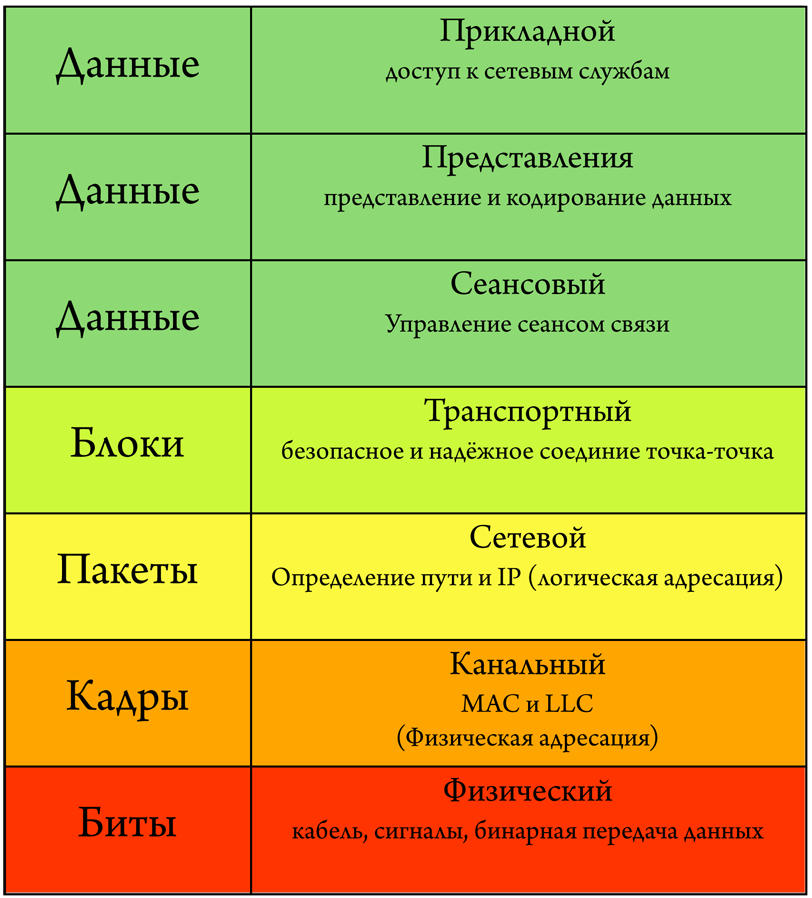
\includegraphics[width=0.4\linewidth]{images/osi}
	\caption{Уровни модели OSI}
	\label{fig:osi}
\end{figure}

В настоящее время двумя самыми популярными протоколами являются \textit{TCP} и \textit{UDP}.
\subsubsection{Уровни модели OSI}
Из \refris{fig:osi} и \cite{kumar_survey_2012} уровни модели OSI делятся на:
\begin{itemize}
	\item \textbf{физический}: предназначен непосредственно для передачи потока данных. Осуществляет передачу электрических или оптических сигналов в кабель или в радиоэфир и, соответственно, их приём и преобразование в биты данных в соответствии с методами кодирования цифровых сигналов;
	\item \textbf{канальный}: полученные с физического уровня данные проверяет на ошибки, если нужно исправляет, упаковывает во фреймы, проверяет на целостность, и отправляет на сетевой уровень;
	\item \textbf{сетевой}: определяет пути передачи данных. Отвечает за трансляцию логических адресов и имён в физические, за определение кратчайших маршрутов, коммутацию и маршрутизацию, за отслеживание неполадок и заторов в сети;
	\item \textbf{транспортный}: организует доставку данных без ошибок, потерь и дублирования (не все) в той последовательности, как они были переданы. Разделяет данные на фрагменты равной величины, объединяя короткие и разбивая длинные (размер фрагмента зависит от используемого протокола);
	\item \textbf{сеансовый}: управляет созданием/завершением сеанса связи, обменом информацией, синхронизацией задач, определением права на передачу данных и поддержанием сеанса в периоды неактивности приложений. Синхронизация передачи обеспечивается помещением в поток данных контрольных точек, начиная с которых возобновляется процесс при нарушении взаимодействия;
	\item \textbf{представления}: на этом уровне может осуществляться преобразование протоколов и сжатие/распаковка или кодирование/декодирование данных, а также перенаправление запросов другому сетевому ресурсу, если они не могут быть обработаны локально;
	\item \textbf{прикладной}: уровень приложений (англ. Application layer). Обеспечивает взаимодействие сети и приложений пользователя, выходящих за рамки модели OSI. На этом уровне работают изученные в работе протоколы автоматизации промышленных сетей.
\end{itemize}
\subsubsection{Транспортный протокол TCP}
\textbf{TCP} \cite{noergaard_chapter_2010} -- один из основных протоколов транспортного уровня. Он обеспечивает надёжную доставку потока байтов от одного устройства к другому. \textit{TCP} ориентирован на качество соединения, а не на скорость. В нём присутствует механизм признания (acknowledgement) и механизм предотвращения скоплений, что уменьшает передачу в то время, как сеть загружена. 

Этот протокол можно назвать стабильным, поскольку он способен адаптироваться к различным ситуациям, происходящим в сети. После отправки пакета в сеть, он сохраняется в буфере и дожидается пакета, подтверждающего получение данных приёмником, что крайне важно при передаче данных с приборов. 

\paragraph{Функции TCP}
\begin{itemize}
	\item \textbf{передача данных}: передаёт непрерывный поток данных в форме сегментов для передачи через сеть;
	\item \textbf{надёжная доставка}: пакеты ACK (см. \refpar{par:tcpstruct}) помогают удостовериться в том, что пакет получен там, где необходимо;
	\item \textbf{управление потоком}: получатель контролирует объём полученных данных при помощи возврата ``окна'' с каждым пакетом ACK. В этом окне содержится то количество данных, которое готов принять приёмник;
	\item \textbf{мультиплексирование}: возможность использовать несколько портов для одновременного обмена данными. Объединение адреса сети и хоста образует \gls{socket}.
\end{itemize}
\paragraph{Структура TCP пакета}\label{par:tcpstruct}
На \refris{fig:pole-tcp} приведена структура TCP.
\begin{figure}[h]
	\centering
	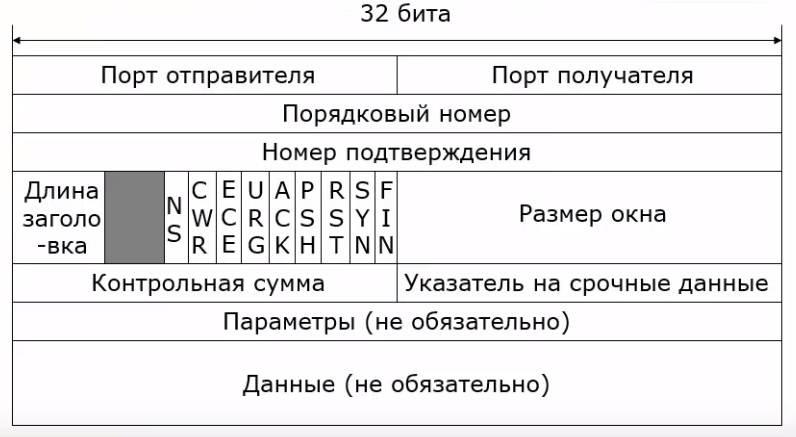
\includegraphics[width=0.8\linewidth]{images/pole-tcp}
	\caption{Структура TCP сегмента}
	\label{fig:pole-tcp}
\end{figure}
Краткое резюме по полям:
\begin{itemize}
	\item \textbf{порт отправителя}: 16-ти битный номер, определяющий отправителя пакета;
	\item \textbf{порт получателя}: 16-ти битный номер, который отправитель использует для отправки пакета получателю;
	\item \textbf{порядковый номер}: в этом поле содержится первый номер байта в сегменте;
	\item \textbf{номер подтверждения (ACK)}: обеспечивает гарантию доставки сообщений. Например, был получен байт $2459$, значит в пакете ACK будет передан следующий ожидаемый байт -- $2460$;
	\item \textbf{длина заголовка}: число 32-х разрядных слов в заголовке;
	\item \textbf{резерв}: 3 - 6 битов, зарезервированные для дальнейшего развития протокола и установлены на значение 0;
	\item \textbf{контрольные биты (флаги)}: определяют использование сегмента или служат проверкой действительности для других полей:
	\begin{itemize}
		\item \textbf{NS}: экспериментальный флаг, используется для защиты от случайного злонамеренного сокрытия пакетов от отправителя;
		\item \textbf{CWR}: используется хостом, чтобы указать, что он получил пакет с установленным флагом \textit{ECE};
		\item \textbf{ECE}: получатель поддерживает ECN (взаимное уведомление хоста и пира о переполнении канала без потери пакетов);
		\item \textbf{URG}: флаг срочности используется для уведомления получателя о необходимости обработки срочных пакетов перед обработкой всех других пакетов. Получатель будет уведомлен, когда будут получены все известные срочные данные. В \reftab{tab:psh-urg} приводится отличие флагов \textit{PSH} и \textit{URG};;
		\item \textbf{ACK}: используется для подтверждения успешного получения пакета;
		\item \textbf{PSH}: используется для информирования отправителя о том, что требуется более высокая пропускная способность, поэтому, если возможно, данные должны передаваться с более высокой пропускной способностью, то есть отправленных пакетов будет больше, однако скорость обмена информацией будет быстрее (что критично для систем реального времени). В \reftab{tab:psh-urg} приводится отличие флагов \textit{PSH} и \textit{URG};
		\begin{table}[b]
			\centering
			\caption{Отличие флагов PSH и URG}
			\label{tab:psh-urg}
			\begin{tabular}{|C{0.4\linewidth}|C{0.4\linewidth}|}
				\hline
				\bfseries PSH & \bfseries URG\\
				\hline
				Все данные из буфера передаются отправителю/приёмнику&Только данные, помеченные флагом \textit{URG} будут переданы приёмнику (немедленно)\\
				\hline
				Данные отправляются последовательно & Данные передаются в случайном порядке\\
				\hline
			\end{tabular}
		\end{table}
		
		\item \textbf{RST}: используется для сброса TCP-соединения при возникновении путаницы в порядковых номерах. В \reftab{tab:fin-rst} приведено отличие \textit{FIN} от \textit{RST};
		\item \textbf{SYN}: флаг синхронизации используется в качестве первого шага в установлении трехстороннего рукопожатия между двумя хостами. Этот флаг должен быть установлен только для первого пакета от отправителя и получателя. На \refris{fig:handshake} показан процесс трехстороннего рукопожатия; 
		\begin{figure}[t]
			\centering
			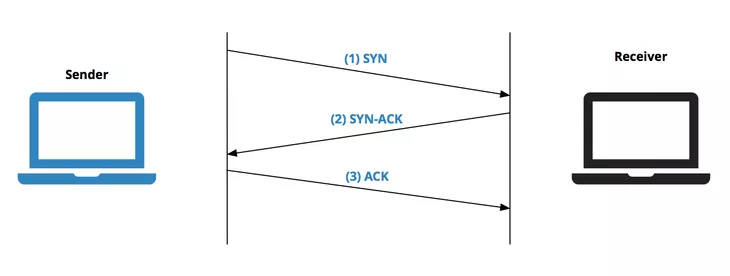
\includegraphics[width=0.8\linewidth]{images/handshake}
			\caption{Трёхстороннее рукопожатие с пакетом SYN}
			\label{fig:handshake}
		\end{figure}
		\item \textbf{FIN}: флаг завершения означает, что от отправителя больше нет данных. Следовательно, он используется в последнем пакете, отправленном отправителем. В \reftab{tab:fin-rst} приведено отличие \textit{FIN} от \textit{RST};
		
		\begin{table}[h]
			\centering
			\caption{Отличие флагов PSH и URG}
			\label{tab:fin-rst}
			\begin{tabular}{|C{0.4\linewidth}|C{0.4\linewidth}|}
				\hline
				\bfseries FIN & \bfseries RST\\
				\hline
				Аккуратно завершает соединение&Резко сообщает другой стороне общения о завершении передачи\\
				\hline
				Нет потери данных & Данные сбрасываются\\
				\hline
				Устройство, получившее этот флаг может продолжать делать запросы & Получатель этого флага должен перестать передавать данные\\
				\hline
			\end{tabular}
		\end{table}
	\end{itemize}
	
	\item \textbf{размер окна}:  в этом поле получатель указывает, сколько данных он может принять. Поле используется для управления потоком;
	\item \textbf{контрольная сумма}: используется для проверки правильности доставки данных, если контрольная сумма, рассчитанная получателем, не совпадает с контрольной суммой в заголовке TCP, то этот сегмент отбрасывается;
	\item \textbf{указатель на срочные данные}: поле указывает порядковый номер октета, которым заканчиваются важные (urgent) данные. Поле принимается во внимание только для пакетов с установленным флагом URG;
	\item \textbf{параметры}: необязательный параметр, применяемый для тестирования и увеличения пропускной способности канала;
	\item \textbf{данные}: сообщение протокола верхнего уровня.
\end{itemize}

\paragraph{Применение TCP}
Технология TCP применяется в следующих областях \cite{kumar_survey_2012}:
\begin{enumerate}
	\item \textbf{HTTP}: самый распространённый протокол передачи данных по сети;
	\item \textbf{FTP}: протокол обмена данными по сети; 
	\item \textbf{IMAP}: доступ к электронной почте;
	\item \textbf{POP}: доступ к электронной почте;
	\item \textbf{RLogin}: удалённый доступ к оборудованию;
	\item \textbf{SMTP}: доступ к электронной почте;
	\item \textbf{SSH}: создание защищённых соединений для удалённого доступа;
	\item \textbf{Modbus TCP}: протокол Modbus, ``завёрнутый'' в оболочку TCP.
\end{enumerate}

\subsubsection{Протокол UDP}
\textbf{UDP} \cite{kumar_survey_2012} -- один из основных протоколов обмена данными. Хост отправляет сообщения в форме датаграммы без предварительной установки соединения. Подходит для случаев, когда важна скорость, а не гарантия доставки. 

\paragraph{Структура UDP датаграммы}
На \refris{fig:udp} приведена структура UDP датаграммы.
\begin{figure}[h]
	\centering
	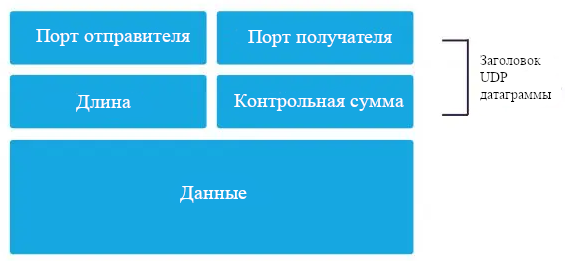
\includegraphics[width=0.8\linewidth]{images/udp}
	\caption{Структура UDP датаграммы}
	\label{fig:udp}
\end{figure}
Краткое резюме по всем полям:
\begin{itemize}
	\item \textbf{source port (порт отправителя)}: порт процесса, который отправляет датаграмму;
	\item \textbf{destination port (порт назначения)}: порт процесса, принимающего датаграмму;
	\item \textbf{length (длина)}: длина датаграммы (вместе с \textit{Header});
	\item \textbf{checksum (контрольная сумма)}: опциональное поле. Контрольная сумма позволяет принимающему устройству проверять целостность заголовка пакета и полезной нагрузки. Это необязательно в IPv4, но стало обязательным в IPv6;
	\item \textbf{data (данные)}: передаваемые пакетом данные.
\end{itemize}
\subsubsection{Сравнение TCP и UDP}
По теоретическим данным \cite{kumar_survey_2012, noergaard_chapter_2010} и экспериментальным данным \cite{hussein_wheeb_performance_2015}, можно сделать следующие выводы: 

\begin{longtable}{|C{8cm}|C{8cm}|}
	\caption{Сравнительная таблица TCP и UDP}
	\label{tab:tcp_udp}\\
	\hline
	\bfseries TCP & \bfseries UDP\\
	\endfirsthead
	\hline
	TCP & UDP\\
	\endhead
	\hline
	Надёжное соединение без перегрузки сети & Не гарантирует надёжность и порядок отправляемых пакетов\\
	\hline
	Создание подключения осуществляется при помощи 3 рукопожатий, см \refris{fig:handshake}. После установки соединения данные передаются в обе стороны \cite{kumar_survey_2012} & Сразу отправляет данные \cite{noergaard_chapter_2010}\\
	\hline
	Пропускная способность \cite{hussein_wheeb_performance_2015} (количество успешно принятых пакетов) у TCP составила $740$ kbps & Пропускная способность \cite{hussein_wheeb_performance_2015} у UDP составила $586$ kbps\\
	\hline
	Задержка у TCP составила $0.059$ ms \cite{hussein_wheeb_performance_2015} & Задержка у UDP составила $0.051$ ms \cite{hussein_wheeb_performance_2015}\\
	\hline
	TCP потерял $8$ пакетов \cite{hussein_wheeb_performance_2015} & UDP потерял $311$ пакетов \cite{hussein_wheeb_performance_2015}\\
	\hline
	TCP доставил $96.92\%$ пакетов \cite{hussein_wheeb_performance_2015} & UDP доставил $74.12\%$ пакетов \cite{hussein_wheeb_performance_2015}\\
	\hline
	TCP применяется там, где необходима надёжность соединения & UDP примняется там, где время играет ключевую роль\\
	\hline
\end{longtable}

\subsubsection{Вывод}
После рассмотрения протоколов транспортного уровня, можно сделать вывод, что для автоматизации вакуумной установки лучше всего пойдёт \textit{TCP}, поскольку в нашем случае важнее не скорость отправки и получения, а надёжность соединения.

Хочется отметить, что хоть TCP и медленнее, но он теряет гораздо меньше пакетов, доставляет куда больший процент пакетов и экономит трафик, поскольку нет необходимости в повторной отравке потерянных пакетов \cite{kumar_survey_2012}. 

Как показала практика, задержки у TCP не сильно выше, чем у UDP \cite{hussein_wheeb_performance_2015}.
\subsection{История разработки промышленных протоколов}
\subsubsection{Предыстория появления автоматизации}
Автоматизация подразумевает в себе соединение воедино различного оборудования. С развитием промышленности требования всё возрастали, что создало спрос на различного вида интерфейсы между измерительным прибором или устройством с системой измерения и управления. К тому же появилась необходимость записи полученных данных \cite{van_gorp_advanced_2009}. 


В течение многих лет системы обмена данными строились вокруг одного мощного вычислительного устройства, к которому шло огромное количество кабелей. Подобная структура была дорога в обслуживании и отличалась низкой степенью автоматизации. 

Альтернативой стали так называемые ЦПС, которые состоят из узлов, обменивающихся данными цифровым способом. На сегодняшний момент таких систем насчитывается большое количество \cite{__2002}.

Уже более 30 лет широко применяется слово \fb. Обычно под этим термином понимается сеть, которая соединяет различного рода устройства (ПЛК, сенсоры) с человеко - машинным интерфейсом (MMI). В это понятие входит множество протоколов, разнообразие которых обусловлено \cite{thomesse_fieldbus_2005}:
\begin{itemize}
	\item нуждой разнообразных компаний из разных областей в средстве сбора и обмена данными в промышленных сетях;
	\item огромному числу разнообразных сенсоров, датчиков и устройств, которые необходимо  было соединить между собой.
\end{itemize}
\subsubsection{Технология Fieldbus: возникновение и требования}
Есть несколько причин возникновения концепта \fb, но их можно разделить на 2 основные группы \cite{thomesse_fieldbus_2005}:
\begin{enumerate}
	\item Потребности пользователей (предприятий):
	\begin{enumerate}
		\item Необходимость единого стандарта;
		\item Концепт предприятия, управляемого компьютерами.
	\end{enumerate}
	\item Возможности технологий:
	\begin{enumerate}
		\item Модель OSI (см. \refris{fig:osi})
		\item Возможности микроэлектроники (внедрение ``интеллекта'' даже в маленькие датчики, ``распределённый интеллект'').
	\end{enumerate}
\end{enumerate}

Последующее развитие индустрии показало, что пользователи выбирают открытые протоколы, поскольку в отличие от проприетарных решений они обладают следующими преимуществами \cite{galloway_introduction_2012}:
\begin{itemize}
	\item большее число поддерживаемого оборудования;
	\item возможность разделить стоимость разработки протокола между компаниями, которые готовы вкладываться в разработку свободного ПО;
	\item качество поддержки открытого ПО обычно выше, чем у проприетарного.
\end{itemize}
\subsubsection{Modbus}
Протокол \mb{} RTU был разработан компанией Modicon (в настоящее время - Schneider Electric) в 1979 году для использования в ПЛК собственного производства. На текущий момент является де - факто стандартом для связи устройств промышленной сети \cite{__2001, van_gorp_advanced_2009}. 

Изначально протокол работал по интерфейсу RS-232, позднее появилась реализации протокола для интерфейсов RS-485 и TCP. Протокол быстро набрал популярность, и многие производители стали внедрять его в своих устройствах.

Позже права на протокол были переданы некоммерческой организации Modbus Organization, которая до сегодняшнего дня владеет стандартом \cite{advantech__2019}.

По распространённости в России конкурирует только с \pb \cite{__2010}. 
\subsubsection{Profibus}
Если протокол \mb{} можно назвать ``дедушкой'' протоколов, то \pb -- ``молодой атлет'': худой и быстрый. Он был разработан в 90-х годах прошлого века для удовлетворения всех потребностей промышленной связи
как для автоматизации производства, так и для автоматизации процессов \cite{powell_profibus_2013}.

\pb настроен как универсальная и открытая (открыт не до конца \cite{__2001}) система связи. Первоначально разработанный для обеспечения дискретного производства, он расширился до автоматизации процессов и корпоративных приложений. \pb включает в себя несколько спецификаций протокола промышленной шины, включая \cite{van_gorp_advanced_2009}:
\begin{itemize}
	\item \textit{Profibus-DP};
	\item \textit{Profibus-PA};
	\item \textit{PROFInet} и другие.
\end{itemize}

Разработавшая его компания Siemens AG до сих пор является основным разработчиком вариаций данной платформы. Несмотря на то, что стандарт позиционируется как открытый, открытыми являются только нижние уровни сетевого взаимодействия. Протоколы доступа к среде, форматы кадров, интерфейсы взаимодействия с приложени­ями прикладного уровня регламентируются проприетарными прото­колами фирмы Siemens. Для получения доступа к ним требуется всту­пление в группу разработчиков стандарта \pb \cite{__2001}.

\subsubsection{Foundation Fieldbus}
\ffb является цифровой системой связи, применяемой в автоматизациии наряду с такими, как \pb и \mb. В настоящий момент включает в себя два протокола информационного обмена между участниками сети \cite{phoenix_contact__2020}: 
\begin{itemize}
	\item H1;
	\item HSE.
\end{itemize}

Стандарт был разработан \textit{American Fieldbus Foundation} в ответ на задержки по созданию международного стандарта \fb \cite{galloway_introduction_2012}. 

Изначально разработанный для решений низкоуровневых задач автоматизации протокол \fb теперь носит название \textit{Fieldbus H1} в связи с появлением таких решений, как:
\begin{itemize}
	\item \textit{Foundation Fieldbus Safety Instrumented Functions} для использования в местах, где необходима безопасность;
	\item\textit{Foundation Fieldbus \Gls{hse}} для работы на высоких скоростях.
\end{itemize}
\subsection{Принципы работы протоколов}
\subsubsection{Понимание термина Fieldbus}\label{par:fieldbus}
В дословном переводе термин \fb означает ``промышленная сеть'', однако это не определённый протокол передачи данных и не тип архитектуры. Под этим термином лучше всего представить сферу применения. 

Промышленная сеть -- это \cite{__2001}:
\begin{itemize}
	\item среда передачи данных, отвечающая жёстким и, зачастую, противоречивым требованиям;
	\item набор стандартных протоколов обмена данными, позволяющих связать воедино оборудование различных производителей, а также обеспечить взаимодействие нижнего и верхнего уровней
\end{itemize}

Обычно \fb -- это двунаправленная цифровая сеть, используемая для контроля и автоматизации. Сеть состоит из \cite{van_gorp_advanced_2009}:
\begin{itemize}
	\item человеко - машинный интерфейс;
	\item главная контролирующая система (master);
	\item набор интерфейсов (slave) между датчиками, насосами, и прочим оборудованием. 
\end{itemize}

Использование подобной системы способно уменьшить время простоя, заранее сообщая диагностические данные оператору. 
\subsubsection{Принцип работы промышленной сети}
\paragraph{Принцип работы промышленной автоматики}
В процессе автоматизации всё делится на 2 уровня. Пример построения такой системы показан на \refris{fig:topology} \cite{promwad__2019}:
\begin{itemize}
	\item \textbf{нижний:} уровень связи устройств управления и подведомственного оборудования (их ещё называют полевые устройства);
	\item \textbf{верхний:} панель управления оператора, через которую он может отслеживать происходящее на объекте автоматизации. Именно на верхнем уровне располагается система управления и автоматизации SCADA \newline (см. \refpar{par:scada}). 
\end{itemize}
\begin{figure}[H]
	\centering
	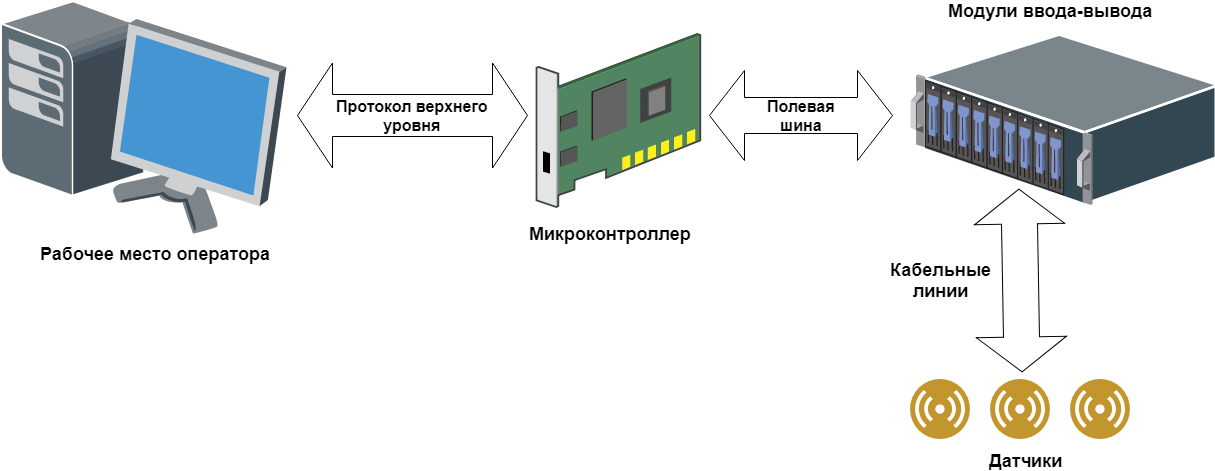
\includegraphics[width=0.9\linewidth]{images/topology}
	\caption{Общая схема автоматизации объекта}
	\label{fig:topology}
\end{figure}
\paragraph{Топология сети}\label{par:topology}
Существует три наиболее значимых топологии сети автоматизации \cite{__2001}. 
\begin{enumerate}
	\item \textbf{Общая шина.} Структура топологии приведена на \refris{fig:shina}.
	\begin{itemize}
		\item \textbf{Достоинства:}
		\begin{itemize}
			\item простая;
			\item недорогая;
			\item лёгкая в настройке;
			\item хорошо подходит для сильно распределённых объектов.
		\end{itemize}
		\item \textbf{Недостатки:}
		\begin{itemize}
			\item присутствие в каждой точке сети общего трафика;
			\item потеря связи при одиночном обрыве канала.
		\end{itemize}
	\end{itemize}
	\begin{figure}
		\centering
		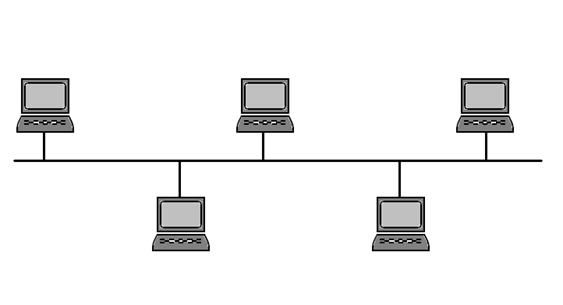
\includegraphics[width=0.5\linewidth]{images/shina}
		\caption{Топология ``общая шина''}
		\label{fig:shina}
	\end{figure}
	\item \textbf{Кольцо.} Структура топологии приведена на \refris{fig:kolco}.
	\begin{itemize}
		\item \textbf{Достоинства:}
		\begin{itemize}
			\item абсолютная предсказуемость трафика;
			\item хорошая пропускная способность.
		\end{itemize}
		\item \textbf{Недостатки:}
		\begin{itemize}
			\item высокая стоимость организации канала связи;
			\item нерациональное использование сетевого трафика при неправильной конфигурации;
			\item потеря всей синхронизации при отключении хотя бы одного из узлов.
		\end{itemize}
	\end{itemize}
	\begin{figure}
		\centering
		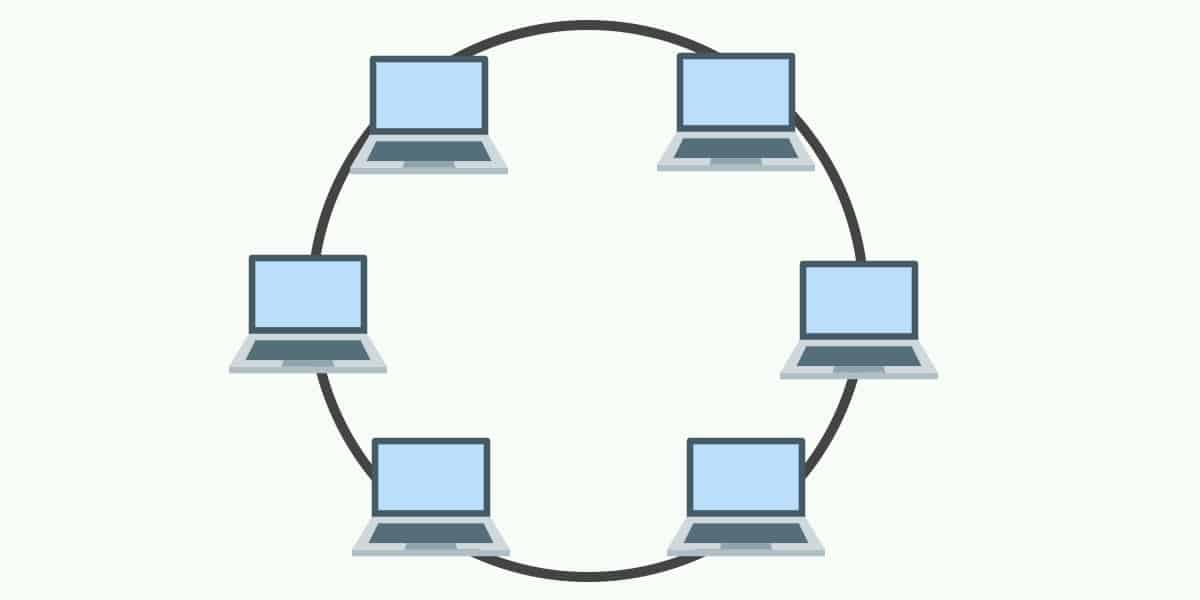
\includegraphics[width=0.5\linewidth]{images/kolco}
		\caption{Топология ``кольцо''}
		\label{fig:kolco}
	\end{figure}
	\item \textbf{Звезда.} Обычно является частью большей сети. Структура топологии приведена на \refris{fig:zvezda}.
	\begin{itemize}
		\item \textbf{Достоинства:}
		\begin{itemize}
			\item дополнительная защита сети от выходи из строя или отключения узлов;
			\item простая масштабируемость;
			\item оптимизация трафика;
			\item допускаются коллизии.
		\end{itemize}
		\item \textbf{Недостатки:}
		\begin{itemize}
			\item обмен идёт через один высоконагруженный компьютер;
			\item потеря связи при одиночном обрыве канала;
			\item ограничение числа рабочих станций числом портов центрального компьютера.
		\end{itemize}
	\end{itemize}
	\begin{figure}
		\centering
		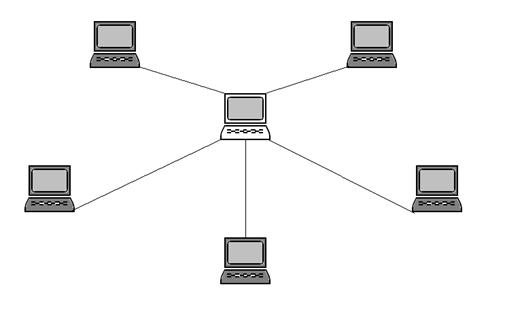
\includegraphics[width=0.5\linewidth]{images/zvezda}
		\caption{Топология ``звезда''}
		\label{fig:zvezda}
	\end{figure}
\end{enumerate}
\paragraph{Основные характеристики сетей}
С развитием техники стало возможным наделить ``интеллектом'' каждый из полевых датчиков. Каждый из узлов цепи способен \cite{__2002}:
\begin{itemize}
	\item принимать команды от других узлов сети;
	\item считывать данные с подключенных датчиков;
	\item оцифровывать полученные данные в случае их представления аналоговым способом;
	\item передавать информацию другим узлам сети.
\end{itemize}
\paragraph{Режимы обмена данными}
В промышленной автоматизации существует три режима обмена данными \cite{__2002, thomesse_fieldbus_2005}:
\begin{enumerate}
	\item \textbf{Ведущий - ведомый.} Ведущее устройство последовательно опрашивает подчинённые узлы. В зависимости от запроса ведомый узел может:
	\begin{itemize}
		\item выполнить полученную команду;
		\item передать ведущему устройству данные с подключенных к нему датчиков.
	\end{itemize}
	Примером таких сетей могуть быть \mb{} и \pb.
	\item \textbf{Клиент - сервер.} Очень похож на предыдущий тип. Клиент запрашивает данные, а сервер их предоставляет. Функции клиента и сервера могуть быть исполнены одним устройством. Отличие от предыдущего пункта -- в отличие от топологии master-slave, топология client-server позволяет серверу автоматически отправлять данные (ведомые устройства этого сделать не могут). Представитель --  \ffb.
	\item \textbf{Подписка.} Узел, нуждающийся в периодическом поступлении информации, подписывается на получение её от другого узла и получает регулярную рассылку без дополнительных запросов. Есть два режима работы:
	\begin{enumerate}
		\item Данные передаются циклически, с определённым интервалом;
		\item Данные передаются только в случае их изменения.
	\end{enumerate}
	Примером такой сети также может быть \ffb.
\end{enumerate}
\subsubsection{Modbus}\label{par:modbus}
\paragraph{Краткое резюме}
Открытый коммуникационный протокол для обмена данными между сетевыми устройствами, основанный на архитектуре ведущий - ведомый (master-slave). Обмен данными представляет собой транзакции, состоящие
из запросов и ответов \cite{__2017-1}. 

\textbf{Достоинства протокола} \cite{__2016}:
\begin{itemize}
	\item открытость;
	\item простота;
	\item массовость;
	\item дешевизна;
	\item отсутствие необходимости в специальных интерфейсных контроллерах \cite{__2010};
	\item надёжный метод контроля ошибок.
\end{itemize}

\textbf{Недостатки протокола}:
\begin{itemize}
	\item невозможность передавать данные по мере получения, необходим постоянный опрос slave - устройств \cite{__2010};
	\item сетевые адреса прописываются на этапе проектирования системы и не могут быть изменены \cite{__2017-1};
	\item длина запроса ограничена, а данные могут быть запрошены только из последовательно расположенных регистров;
	\item не предусмотрен способ, с помощью которого подчиненное устройство могло бы обнаружить потерю связи с ведущим;
	\item соответствие регистров типам измерений и измерительным каналам не регламентировано, что может приводить к несовместимости протоколов
	счетчиков разных типов даже одного производителя;
	\item нет защиты от сторонних несканционированных команд, нельзя передавать конфиденциальные данные \cite{_modbus_2021}.
\end{itemize}

\paragraph{Принцип работы}
\subparagraph{Физический уровень}
Протокол \mb может быть использован со следующими интерфейсами:
\begin{itemize}
	\item \textbf{RS-232/422/485}:  последовательные интерфейсы, широко распространенные в промышленности. Интерфейсы RS-422/485 обеспечивают дальность сигнала до 1200 метров. Используются протоколы \mb RTU/ASCII
	\item \textbf{TCP/IP}: физическим каналом передачи данных могут любые ethernet-ин\-терфейсы. Используется протокол \mb \tcp.
\end{itemize}
Существует 3 разновидности протокола \mb{} \cite{_modbus_2021}:
\begin{enumerate}
	\item \mb{} \textit{ASCII}: в котором данные кодируются символами из таблицы ASCII (рис. 1) и передаются в шестнадцатеричном формате и данный формат протокола встречается довольно редко;
	\item \mb{} \textit{RTU}: самый распространенный вариант протокола \mb, который кодирует данные в двоичном формате и разделяет пакеты с помощью временного интервала;
	\item \mb{} \textit{TCP}:  данные кодируются в двоичном формате и упаковываются в TCP - пакет, для передачи по IP-сетям и предназначен для работы в локальных сетях.
\end{enumerate}

На \refris{fig:modbusphys} показан пример построения схемы контроля за неким объектом при помощи протокола \mb{} \cite{advantech__2019}.

\begin{figure}[p]
	\centering
	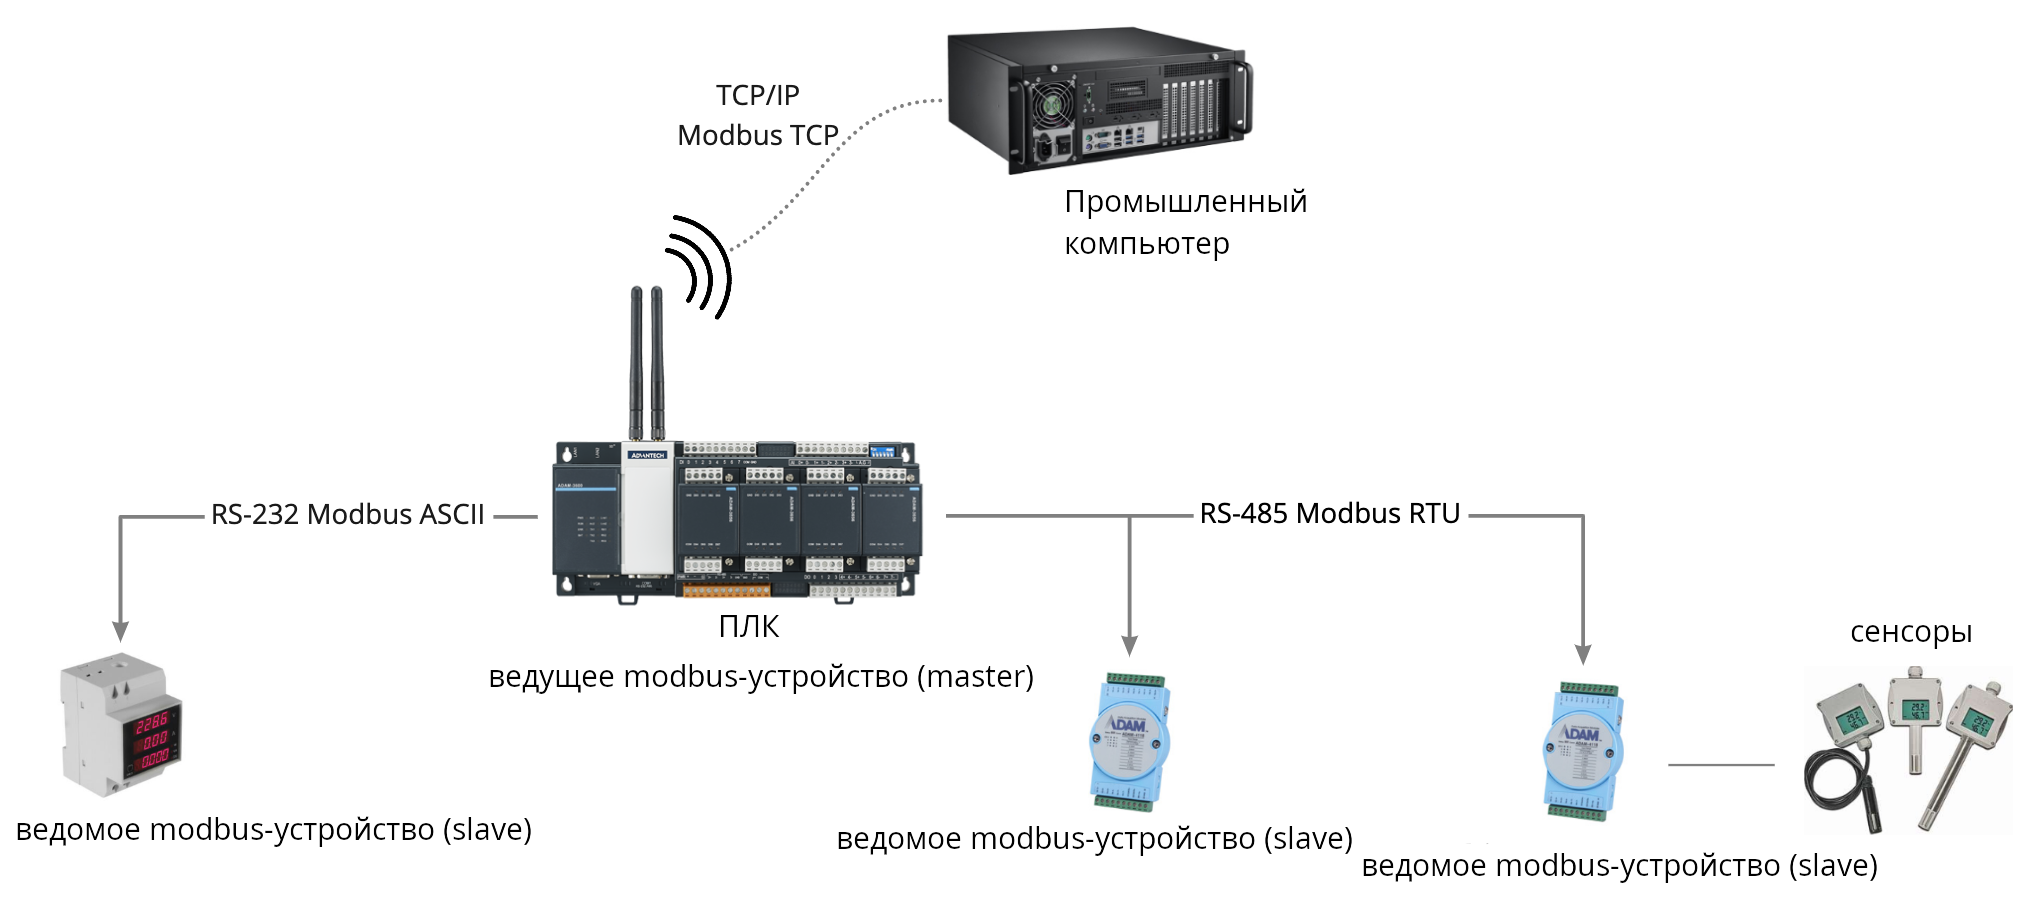
\includegraphics[width=0.9\linewidth]{images/modbus_phys}
	\caption{Физический уровень протокола \mb{}}
	\label{fig:modbusphys}
\end{figure}

\subparagraph{Логический (канальный) уровень}
Протокол \mb предполагает $1$ ведущее устройство и до $247$ ведомых. Обмен данными начинается ведущим устройством. Ведомые не могут начинать передачу и обмениваться данными между собой. В любой момент времени может происходить только один акт обмена. Структуры пакетов \mb при работе 3 способами приведены на \refris{fig:modbusstruct}.
\begin{figure}[p]
	\centering
	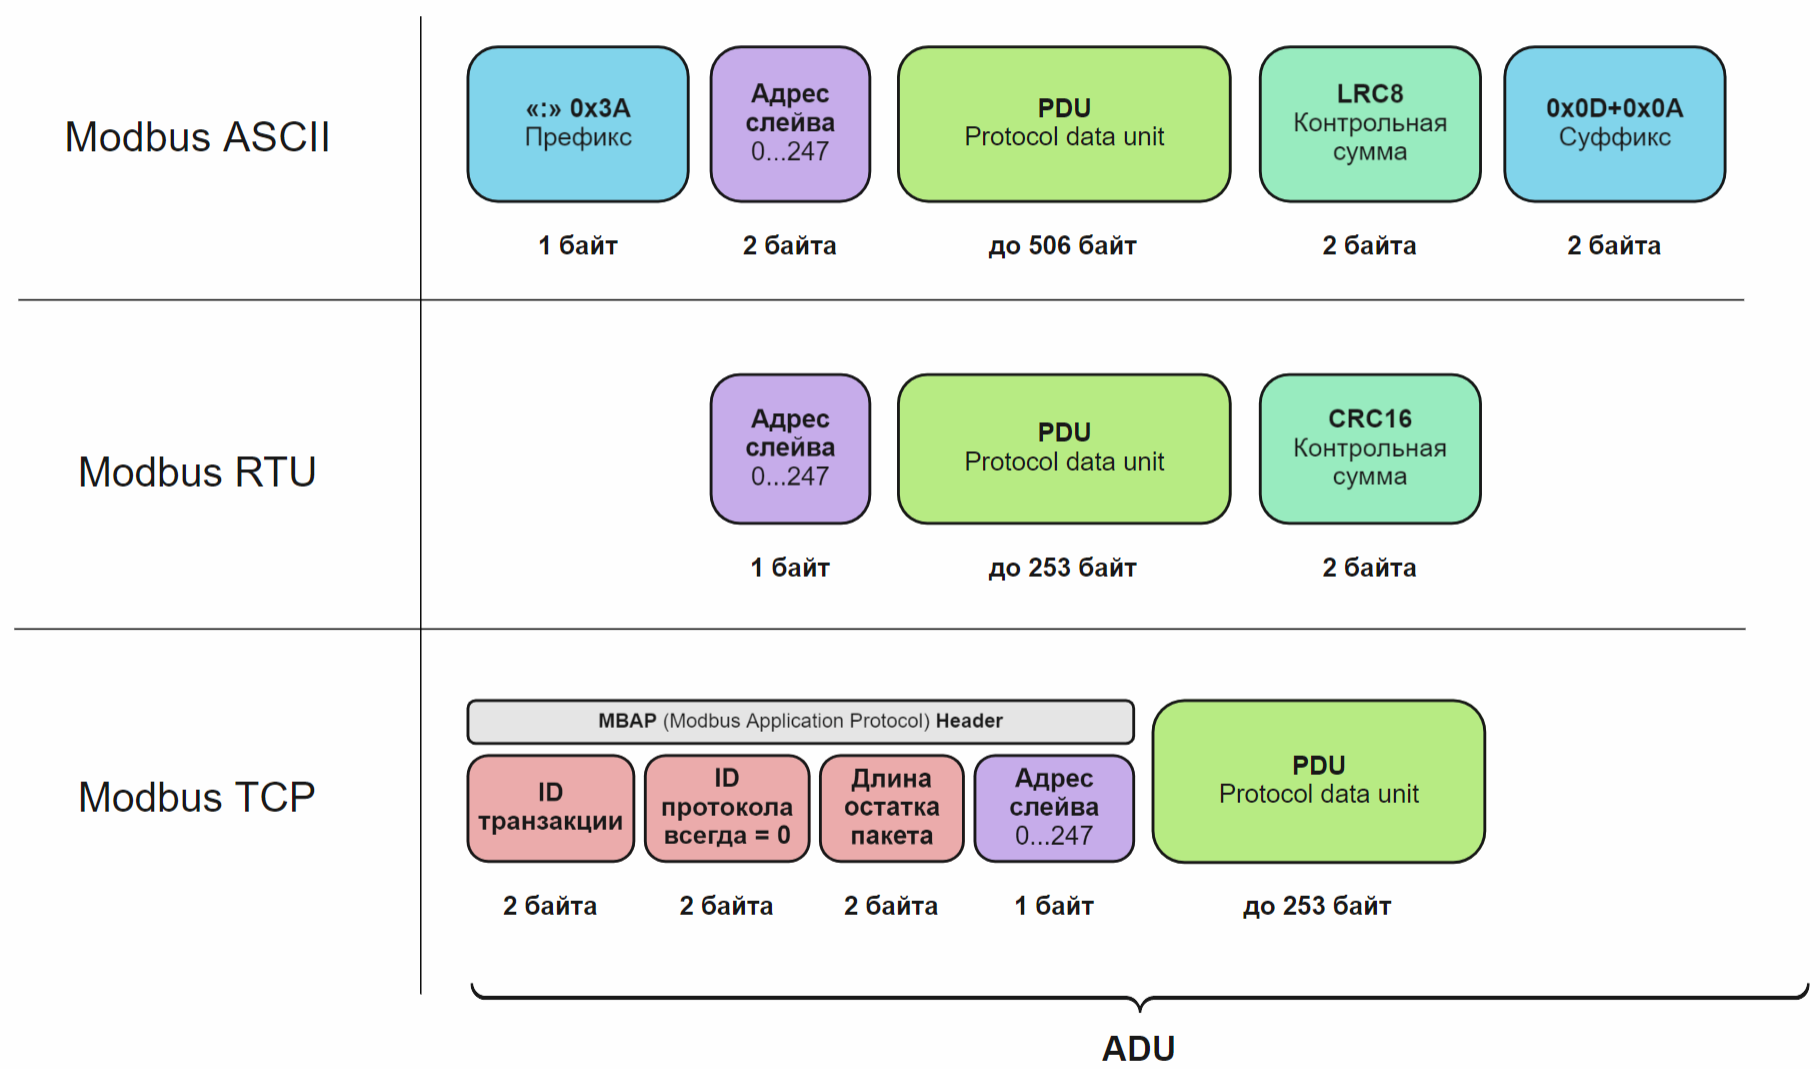
\includegraphics[width=0.9\linewidth]{images/modbus_struct}
	\caption{Структура пакета \mb}
	\label{fig:modbusstruct}
\end{figure}


\subparagraph{Modbus RTU} \label{par:modbusrtu}
Сообщение начинает восприниматься как новое после паузы длиной в $14$ бит. На \refris{fig:modbuspdu} показан формат пакета.
\begin{figure}
	\centering
	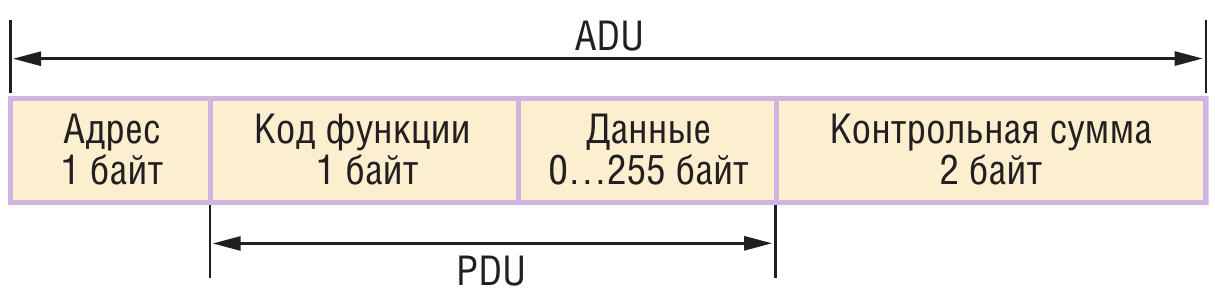
\includegraphics[width=\linewidth]{images/modbus_PDU}
	\caption{Формат кадра протокола \mb \textit{RTU}}
	\label{fig:modbuspdu}
\end{figure}
У пакета есть следующие поля \cite{__2010}:
\begin{itemize}
	\item \textbf{Адрес:} содержит адрес ведомого устройства. Адрес отправляется даже при ответе на запрос мастера, тем самым всегда понятно, откуда пришёл ответ;
	\item \textbf{Код функции:} говорит модулю о том, что ему необходимо сделать;
	\item \textbf{Данные:} тут может содержаться информация о параметрах, которые используются в исполнении команд мастера или показания, передаваемые мастеру;
	\item \textbf{Контрольная сумма:} используется для проверки целостности пакета.
\end{itemize}

\subparagraph{Modbus TCP}
Данный протокол используется для того, чтобы подключить устройства, работающие по протоколу \mb к сети \textit{Internet} \cite{__2018-1}. То есть, в соответствии со стандартом \osi (см. \refris{fig:osi}) на транспортном уровне используется протокол \tcp, а на прикладном -- \mb. В этом случае проверка целостности пакета ложится на протокол \tcp. Структура протокола \mb \tcp приведена на \refris{fig:modbustcp}. 
\begin{figure}
	\centering
	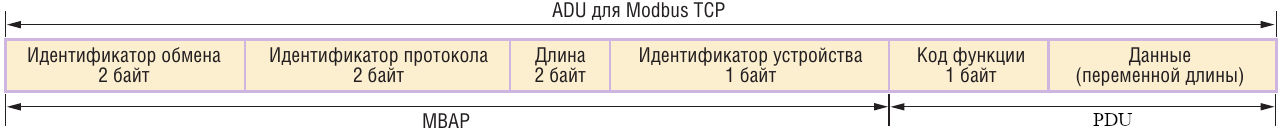
\includegraphics[width=1\linewidth]{images/modbus_TCP}
	\caption{Формат кадра протокола \mb \tcp}
	\label{fig:modbustcp}
\end{figure}
У пакета есть следующие поля \cite{__2010}:
\begin{itemize}
	\item \textbf{Идентификатор обмена:} используется для идентификации сообщения в случае,	когда в пределах одного TCP - соединения клиент посылает серверу несколько сообщений без ожидания ответа после каждого сообщения;
	\item \textbf{Идентификатор протокола:} всегда выставлен на 0 (как и у протокола \tcp);
	\item \textbf{Длина:} указывает количество следующих байтов;
	\item \textbf{Идентификатор устройства:} адрес slave - устройства;
	\item \textbf{Код функции:} аналогично \refpar{par:modbusrtu};
	\item \textbf{Данные:} аналогично \refpar{par:modbusrtu}.
\end{itemize}

Как можно заметить, \mb \textit{RTU} оказывается ``вшит'' в пакет \tcp, тем самым получается \mb \tcp. На \refris{fig:modbustcp_ip} показан принцип работы такой системы \cite{__2010}:
\begin{itemize}
	\item коды функций передаются с прикладного уровня на транспортный (\mb -- \tcp), добавление заголовка \tcp;
	\item передача на сетевой уровень, добавление блока \textit{IP};
	\item передача на канальный уровень, а затем на физический (\textit{Ethernet})
\end{itemize}
После прохождения через канал связи пакет начинает обратное движение согласно модели \osi (см. \refris{fig:osi}). 
\begin{figure}[h]
	\centering
	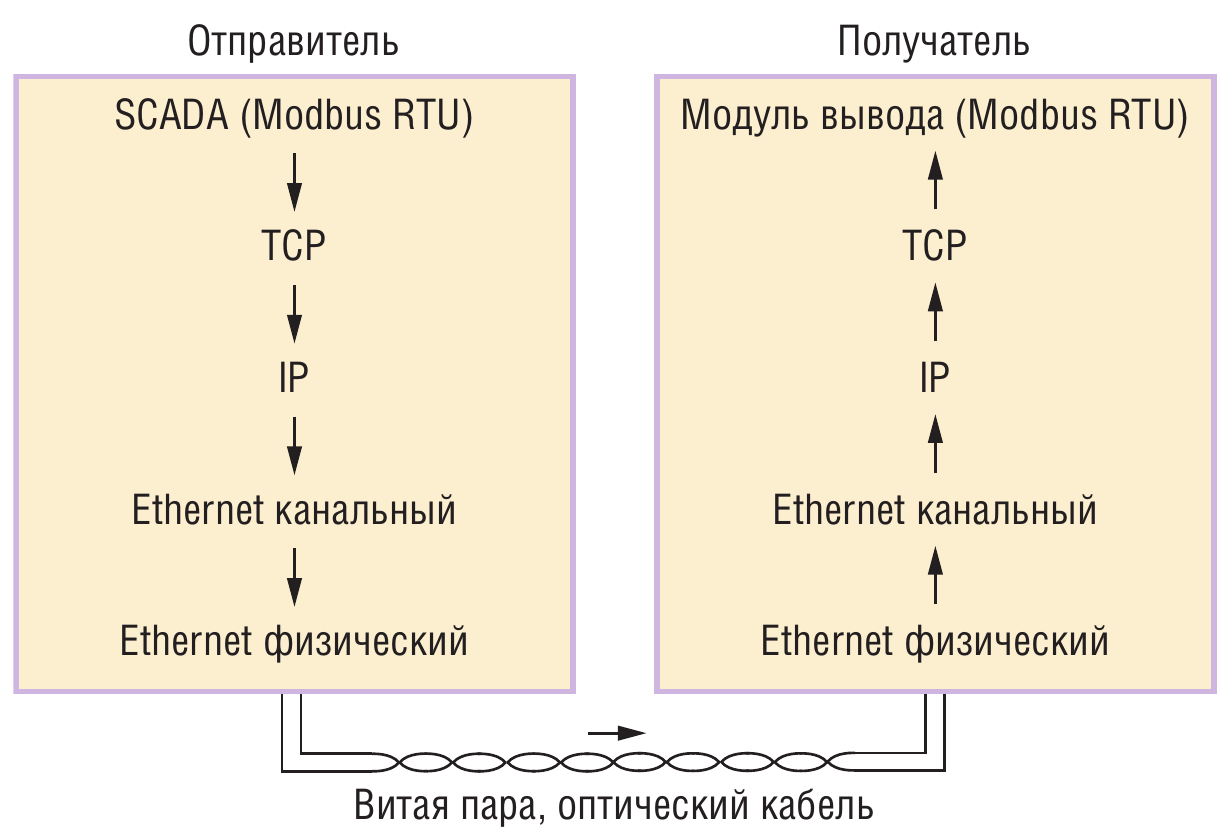
\includegraphics[width=0.7\linewidth]{images/modbus_tcp}
	\caption{Процесс передачи пакетов \mb \textit{RTU} по сети \tcp}
	\label{fig:modbustcp_ip}
\end{figure}


Более подробно о работе с протоколом \mb{} можно узнать в документации \cite{swales_open_1999}. 
\subsubsection{Profibus}\label{par:profibus}
\paragraph{Краткое резюме}
\pb -- один из самых популярных и широко применяемых протоколов при автоматизации. Протокол работает по такой же системе, что и \mb: master -  slave. 

Этот протокол используется для передачи полевых данных в системы уп\-равления технологическими процессами и обеспечивает прямое управление и обслуживание устройств. При смене полевого устройства новое устройство автоматически берет на себя роль предыдущего устройства, что позволяет легко осуществлять смену устройств без прерывания работы системы.

Существует 3 подвида \pb \cite{__2001, __2002, galloway_introduction_2012}:
\begin{enumerate}
	\item \pb \textit{DP}: быстрый протокол с одним мастером. Обеспечивает высокую скорость передачи данных (до $12$ Мбит/с). Отлично подходит для построения систем контроля и сбора данных с одним ведущим узлом. Работает на низком уровне;
	\item \pb \textit{FMS}: предназначен для работы с системами производителей, не поддерживающих \pb \textit{DP} \cite{__2001, promwad__2019-1};
	\item \pb \textit{PA}: используется во взрывоопасных местах. Подключается к \newline \pb \textit{DP} через разветвители.
\end{enumerate}
\paragraph{Принцип работы}\label{par:pb_work}
\pb как и \mb работает по протоколу master - slave. Однако, в отличие от \mb, этот протокол способен работать с несколькими мастерами благодаря кольцевой топологии (см. \refpar{par:topology}) и маркерному доступу \cite{powell_profibus_2013}.

Каждое устройство должно пройти через ``инициализацию'', во время которой оно подключается к сети. У каждого ведомого устройства есть ``таймер отказоусточивости'' -- если мастер не разговариал с ним некоторое время, устройство возвращается в ``спячку'' и ему придётся повторить процедуру инициализации снова. В комбинации со сторожевым таймером это даёт гарантию того, что передача данных будет происходить каждый ``цикл''.

Цикл проходит так (см. \refris{fig:profibustoken}): мастер А получает токен, опрашивает своих подопечных и передаёт токен дальше. 

\begin{figure}
	\centering
	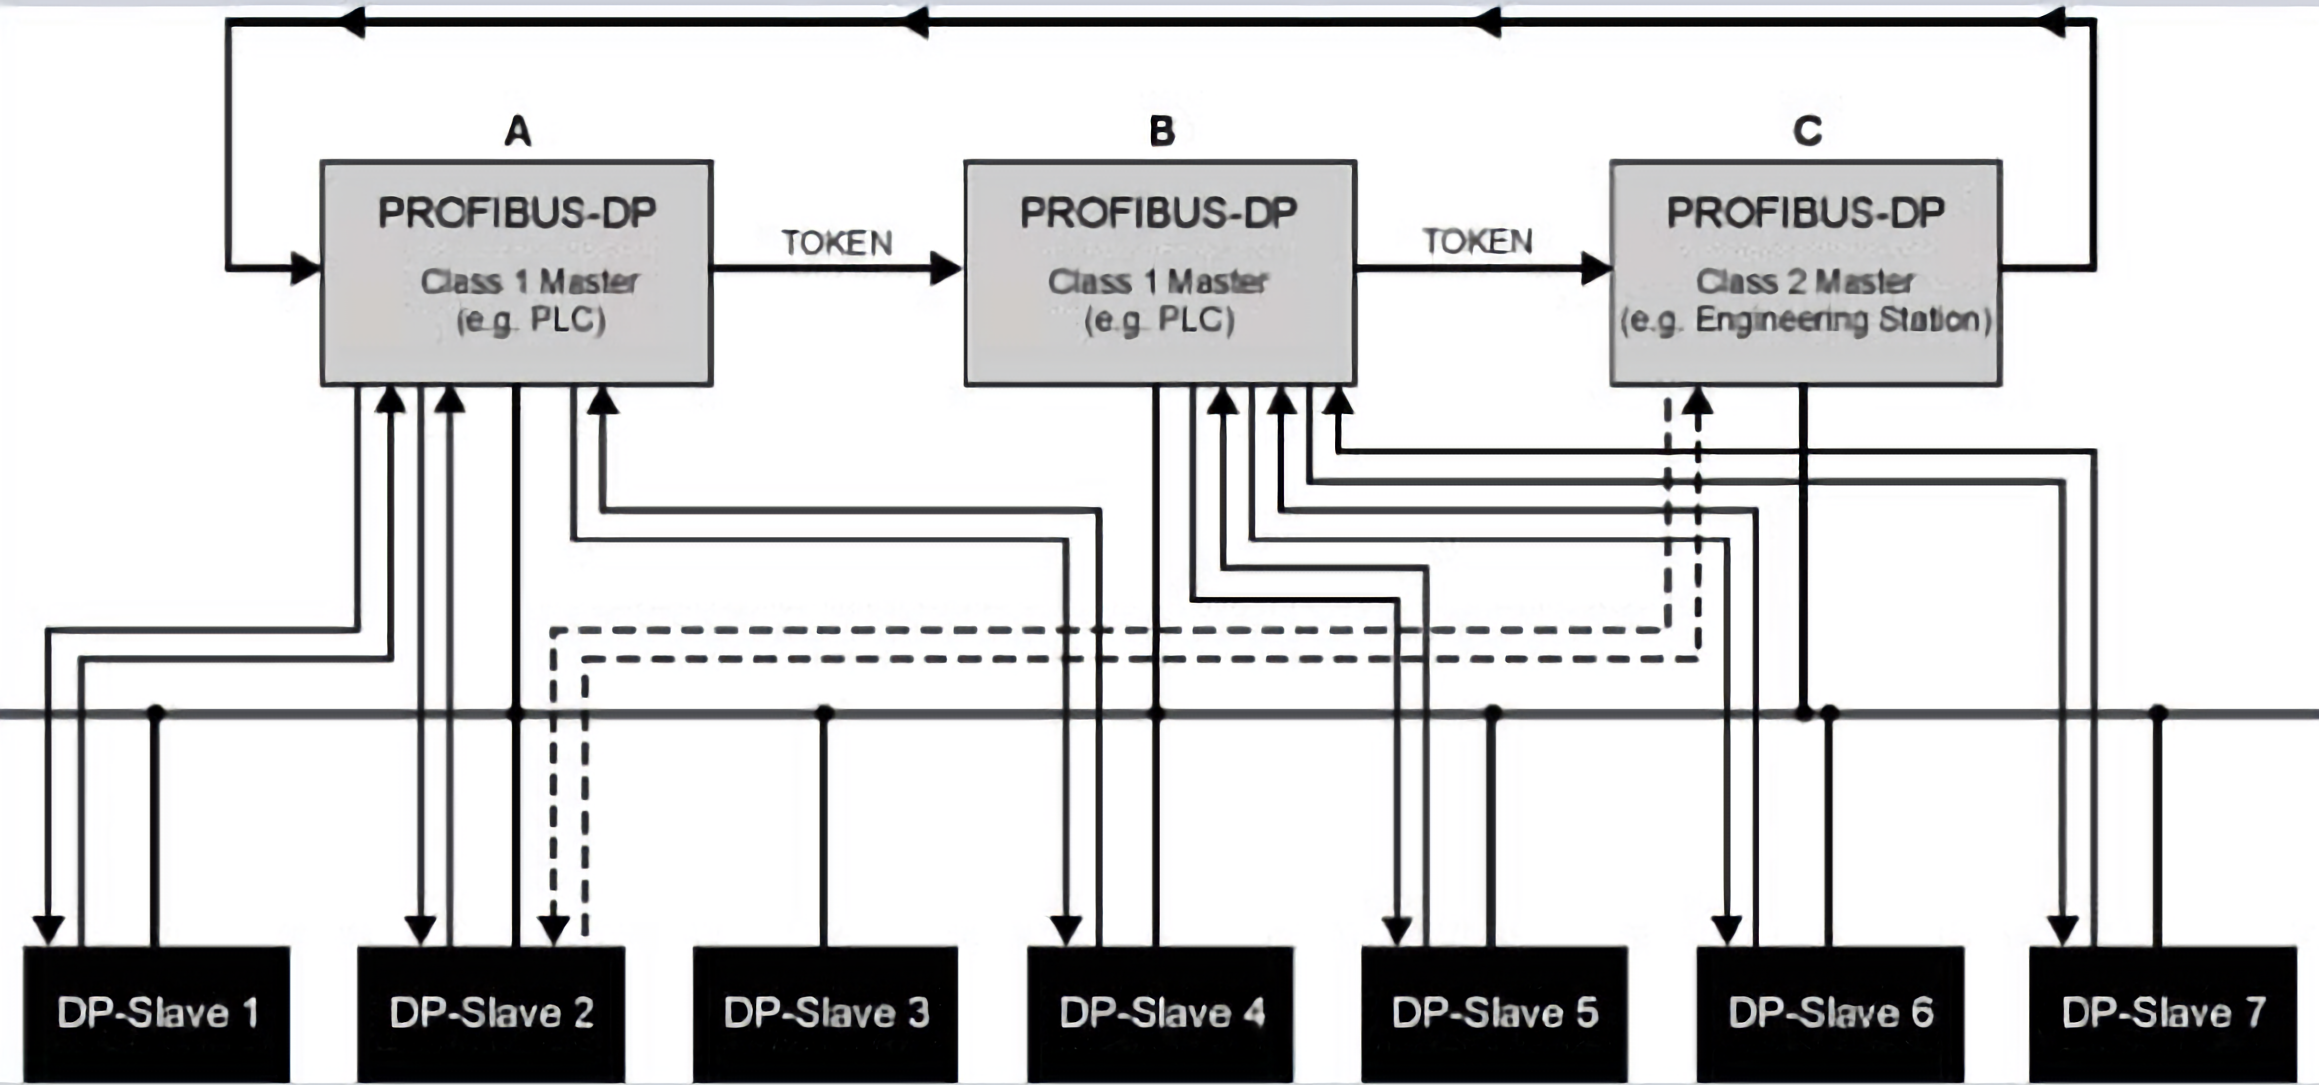
\includegraphics[width=0.9\linewidth]{images/profibus_token}
	\caption{Цикл \pb}
	\label{fig:profibustoken}
\end{figure}

\subparagraph{Физический уровень}
На физическом уровне \pb использует стандарт RS-485 при скорости передачи до 12 Мбит/с и с размерами сегментов сети до 32 устройств. Количество устройств можно увеличить с помощью повторителей интерфейса \cite{powell_profibus_2013}.

Протокол устойчив к помехам и шумам. В случае правильной установки и настройки представляет из себя сверхнадёжную систему \cite{powell_profibus_2013}.

\subparagraph{Канальный уровень}
Обеспечиваются следующие требования:
\begin{itemize}
	\item в процессе коммуникации между ведущими устройствами необходимо обеспечить выполнение каждым из них своей задачи в течение заранее определенного интервала времени;
	\item взаимодействие ведущих устройств (контроллеров) с ведомыми должно происходить максимально быстро.
\end{itemize}

Используемый в протоколе метод передачи маркера по кольцу показан на \refris{fig:profibustoken}.
\subparagraph{Передача сообщений}
У \pb есть два типа сервисов передачи сообщений \cite{__2015}:
\begin{enumerate}
	\item \textbf{SRD}: позволяет отправить и получить данные в одном цикле обмена. Этот способ обмена наиболее распространен в \pb и очень удобен при работе с устройствами ввода-вывода, поскольку в одном цикле можно и отправить и получить данные;
	\item \textbf{SND}: используется, когда надо отправить данные одновременно группе ведомых устройств (многоабонентский режим) или всем ведомым устройствам (широковещательный режим). При этом ведомые устройства не отправляют свои уведомления мастеру.
\end{enumerate}

Пакет данных в \pb называется телеграмма. Её структура приведена на \refris{fig:profibustg}
\begin{figure}
	\centering
	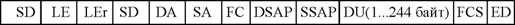
\includegraphics[width=\linewidth]{images/profibus_tg}
	\caption{Структура телеграммы \pb}
	\label{fig:profibustg}
\end{figure}
Расшифровка полей телеграммы \cite{__2015, acromag_introduction_2002}:
\begin{itemize}
	\item \textbf{SD:} стартовый разделитель. Используется для указания начала телеграммы и ее формата;
	\item \textbf{LE:} длина передаваемых данных (DA+SA+FC+DSAP+SSAP+DU);
	\item \textbf{LEr:} повторение поля LE с целью его резервирования;
	\item \textbf{DA:} адрес устройства-получателя телеграммы;
	\item \textbf{SA:} адрес отправителя;
	\item \textbf{FC:} код типа телеграммы (запрос, уведомление, ответ, диагностические данные, тип устройства - мастер или ведомый, приоритет, уведомление);
	\item \textbf{DSAP:} устройство-получатель использует это поле, чтобы определить, какой тип сервиса нужно выполнить;
	\item \textbf{SSAP:} COM порт отправителя;
	\item \textbf{DU:} данные длиной от 1 до 244 байт;
	\item \textbf{FCS:} контрольная сумма телеграммы (сумма значений полей DA+SA+ FC+DU, по модулю 255);
	\item \textbf{ED:} признак конца.
\end{itemize} 

\paragraph{Profinet}
Как и у \mb, у \pb есть аналог для работы с сетью. Только в отличие от инкапсулирования обычного пакета в \tcp, \textit{Profinet} -- протокол, который был разработан для того, чтобы использовать все преимущества сети \textit{Ethernet} (включая такую функцию, как \textit{Profisafe}) \cite{powell_profibus_2013}.

Более подробно с протоколами семейства \pb можно ознакомиться в документации стандарта \cite{acromag_introduction_2002}.
\subsubsection{Foundation Fieldbus}\label{par:ffbus}
Один из самых молодых протоколов, появился в $1995$ как результат консорциума крупных производителей в ответ на задержки в разработке единого стандарта ``полевой шины'' \cite{galloway_introduction_2012}.

Многим этот протокол схож с \pb \textit{PA} \cite{__2002} :
\begin{itemize}
	\item работа во взрывоопасных зонах;
	\item передача сигнала вместе с питанием.
\end{itemize}
\ffb{} -- двухуровневый сетевой протокол, который \cite{__2001}:
\begin{itemize}
	\item объединяет компьютеры верхнего уровня;
	\item объединяет датчики, контроллеры, исполнительные механизмы.
\end{itemize}

К самым главным \textbf{преимуществам} стандарта можно отнести \cite{__2002, noauthor_foundation_2001}:
\begin{itemize}
	\item \ffb{} -- открытый протокол, для связи и создания приложений контроля;
	\item протокол делает ставку на распределённый интеллект, а не на центральный аппарат.  \ffb ориентирован на обеспечение одноранговой связи между узлами без центрального ведущего устройства. Этот подход даёт возможность реализовать системы управления, распределенные не только физически, но и логически, что во многих случаях позволяет повысить надежность и живучесть автоматизированной системы;
	\item все устройства, работающие по протоколу \ffb, должны работать между собой вне зависимости от производителя без дополнительных ухищрений;
	\item существует специальный язык описания оконечных устройств (DDL), позволяющий легко расширять сеть. Достаточно физически подключить новое устройство, и оно	тут же самоопределится на основании заложенного описания DD, после чего все функциональные возможности нового узла становятся доступными в сети.
\end{itemize}
Однако, у протокола есть и существенный недостаток:
\begin{itemize}
	\item малая распространённость в России, где конкурируют только \mb и \pb. 
\end{itemize}









\subsection{SCADA-системы}\label{par:scada}
\subsubsection{Что такое SCADA - система}
\Gls{scada} -- \glsdesc{scada} \cite{daneels_what_1999}.

Понятие SCADA - система включает в себя \cite{__2019}:
\begin{itemize}
	\item комплекс программ разработки ПО для обеспечения систем автоматизации;
	\item \Gls{pak} систем управления процессом, который осуществляет контроль и сбор данных.
\end{itemize}
\subsubsection{Задачи SCADA - систем}
Современная SCADA - система должна решать такие задачи, как \cite{daneels_what_1999, __2019, __2013-1}:
\begin{itemize}
	\item обмен данными с контроллерами, платами вывода и прочими устройствами (желательно в реальном времени);
	\item обработка полученной информации;
	\item отображение информации на \gls{mmi};
	\item ведение базы данных;
	\item аварийная сигнализация и управление тревожными сообщениями;
	\item связь с приложениями во внешней среде;
	\item автоматическое управление и корректирование в связи с изменением условий процесса;
	\item обеспечение оператора языком программирования для составления запросов к оборудованию;
	\item иметь в себе драйвера всех подключаемых устройств.
\end{itemize}
\subsubsection{Структура системы}
Структуру современной SCADA - системы можно описать так (см. \refris{fig:scadasys}): оборудование/датчики передают данные на ПЛК, которые отправляют данные оператору на \gls{mmi} (\glsdesc{mmi}).

\begin{figure}[p]
	\centering
	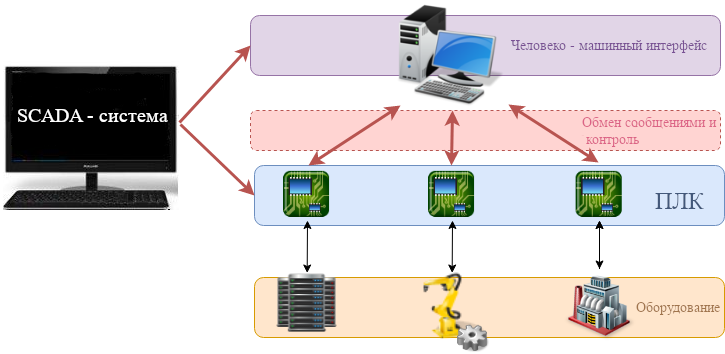
\includegraphics[width=\linewidth]{images/scadasys}
	\caption{Топология SCADA - системы}
	\label{fig:scadasys}
\end{figure}


\subsubsection{Пример применения SCADA систем}
SCADA - системы применяются во всех отраслях промышленности. На \refris{fig:at-genie} показана SCADA - система компании Advantech.


\begin{figure}[p]
	\centering
	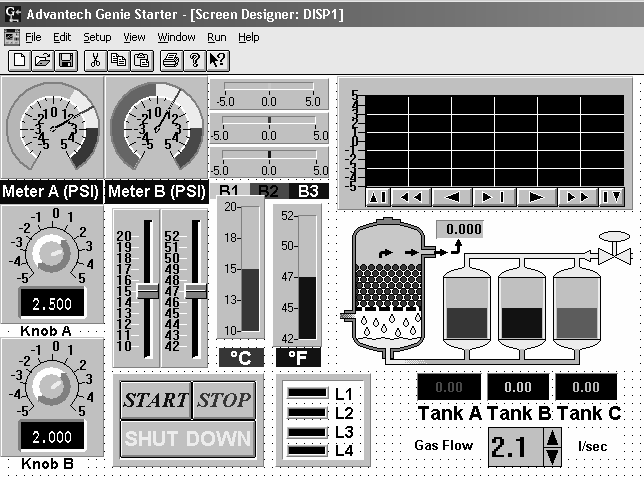
\includegraphics[width=\linewidth]{images/at-genie}
	\caption{SCADA - система Advantech Genie}
	\label{fig:at-genie}
\end{figure}

\subsection{Сравнение протоколов передачи данных промышленных сетей}
В \refpar{par:modbus}, \refpar{par:profibus} и \refpar{par:ffbus} были рассмотрены 3 протокола передачи данных для промышленных сетей.

Сравнение будет проводиться только среди \mb и \pb, поскольку хоть \ffb и является самым популярным протоколом с открытым стандартом и множеством возможностей, она не так широко распространена в мире и России, нет достаточной поддержки оборудования \cite{__2001, _foundation_1999}. 

\subsubsection{Modbus}
\noindent Особенности:
\begin{itemize}
	\item 3 разновидности: TCP, TRU и ACII;
	\item имеется контрольная сумма для проверки целостности;
	\item технология master - slave, только одно ведущее звено;
	\item максимум 32 устройства в сети (64 с повторителями).
\end{itemize}
Достоинства \cite{van_gorp_advanced_2009}:
\begin{itemize}
	\item хорошая документация;
	\item открытость;
	\item большое число поддерживаемых устройств.
\end{itemize}
Недостатки:
\begin{itemize}
	\item нет возможности диагностировать проблемы с устройствами, если такие случаются;
	\item некоторые производители могут добавить ``от себя'' и весь смысл стандартизации теряется.
\end{itemize}
\subsubsection{Profibus}
\noindent Особенности:
\begin{itemize}
	\item может иметь несколько ведущих звеньев, передающих важность при помощи маркера (см. \refpar{par:pb_work});
	\item имеется контрольная сумма для проверки целостности;
	\item технология master - slave;
	\item максимум 127 устройств;
	\item все устройства проходят сертификацию, поэтому совместимы без дополнительных ухищрений.
\end{itemize}
Достоинства:
\begin{itemize}
	\item поддержка цифрового и аналогового форматов;
	\item поддержка нескольких ведущих звеньев;
	\item простая масштабируемость и лёгкое добавление новых устройств.
\end{itemize}
Недостатки:
\begin{itemize}
	\item стандарт открыт не полностью (см. \cite{__2020});
	\item сложнее в освоении, чем \mb;
	\item в СНГ \mb более популярен.
\end{itemize}
\subsubsection{Итог}
Несмотря на все достоинства протокола \pb, описанные в \cite{powell_profibus_2013}, выбор пал на протокол \mb \tcp в связи с:
\begin{enumerate}
	\item Простой документацией;
	\item Полной открытостью;
	\item Наличием в современных средах разработки поддержки протокола \tcp (что облегчает работу с протоколом \mb \tcp);
	\item Оборудованием ОВЕН, работающем по протоколу \mb.
\end{enumerate}
\subsection{Примеры применения протокола Modbus для автоматизации}
Протокол применятся в разнообразных сферах деятельности человека:
\begin{enumerate}
	\item Передача показаний приборов учёта \cite{__2016};
	\item Автоматизация вакуумной установки \cite{__2017}. Исследование показало, что автоматизация установки минимизирует количество ошибок оператора, тем самым повышается надёжность процесса и облегчается работа оператора;
	\item Мониторинг теплиц, мониторинг системы нагрева воды солнечной энергией \cite{advantech__2019}.
\end{enumerate}
\subsection{Преимущества автоматизации}
К преимуществам автоматизации можно отнести:
\begin{itemize}
	\item уменьшение количества ошибок оператора;
	\item упрощение контроля за процессом;
	\item повышение надёжности процесса.
\end{itemize}
\subsection{Дальнейшая работа}
На основе проведённой научной работы и выбора протоколов передачи данных для автоматизации технологического процесса необходимо изучить одну из современных сред разработки, которая позволяет использовать все возможности протоколов \mb и \tcp.
	\begin{center}
	\normalsize\bfseries\MakeUppercase{выводы и результаты}
\end{center}
\addcontentsline{toc}{section}{ВЫВОДЫ И РЕЗУЛЬТАТЫ}

\begin{enumerate}
	\item Был составлен терминологический словарь, сформированы поисковые запросы и найдена литература по промышленным протоколам и автоматизации;
	\item В результате проведённого литературного обзора были изучены два самых популярных сетевых протокола обмена данными: 
	\begin{itemize}
		\item TCP;
		\item UDP.
	\end{itemize}
Был выбран протокол \tcp, поскольку он:
\begin{itemize}
	\item ориентирован на качество соединения, а не на скорость;
	\item проверяет пакеты на целостность;
	\item имеет задержку передачи данных не сильно ниже, чем у \textit{UDP}, который славится своей быстротой;
	\item не нагружает канал, поскольку отправляет новый пакет только после подтверждения получения предыдущего.
\end{itemize}
	\item Были проанализированы три протокола промышленных сетей: 
	\begin{itemize}
	    \item \mb;
	    \item \pb;
	    \item \ffb.
	\end{itemize}
По результатам анализа всех трёх протоколов был выбран \mb, поскольку он:
\begin{itemize}
	\item прост в освоении;
	\item проверен временем и поддерживается большим числом производителей;
	\item является полностью открытым стандартом (в отличие от \pb);
	\item является наиболее распространённым (в странах СНГ протокол \textit{Foun\-dation Fieldbus}, несмотря на свои преимущества, не используется).
\end{itemize}
	\item Сделаны выводы о преимуществах автоматизации:
	\begin{itemize}
		\item уменьшение количества ошибок оператора;
		\item упрощение контроля за процессом;
		\item повышение надёжности процесса.
	\end{itemize}
	\item Была начата разработка собственной системы управление и контроля \newline SCADA.
\end{enumerate}
\newpage

\begin{center}
	\normalsize\bfseries\MakeUppercase{заключение}
\end{center}
\addcontentsline{toc}{section}{ЗАКЛЮЧЕНИЕ}

Технологии плотно вошли во все сферы нашей жизни. Не обходится без них и промышленность: благодаря наработкам \textit{IT}-индустрии мы имеем огромное количество протоколов обмена данными между устройствами и большое число промышленных протоколов, среди которых можно выделить три самых популярных:
\begin{enumerate}
	\item \mb;
	\item \pb;
	\item \ffb. 
\end{enumerate}

Промышленные протоколы используются при построении SCADA-систем для контроля за процессом производства. Эти системы помогают избежать таких недостатков ручного управления, как:
\begin{itemize}
	\item простой оборудования в связи с отсутствием оператора;
	\item уменьшение производительности в связи с необходимостью ручного управления;
	\item ухудшение качества продукции в связи с неточным следованиям инструкциям.
\end{itemize}

По результатам работы, проделанной в дисциплине <<Научно-исследовательс\-кая работа>>, была начата разработка собственной SCADA-системы при помощи библиотек Qt.

	\nocite{*}
	%\printbibliography[heading=bibintoc]
	\addcontentsline{toc}{section}{\bibname}
	\printbibheading
	\printbibliography[filter=papers,heading=subbibliography,title={Научные статьи}]
	\printbibliography[type=online,heading=subbibliography,
	title={Онлайн-издания}]
	\printbibliography[type=incollection,heading=subbibliography,
	title={Разделы книг}]
	\printbibliography[type=book, heading=subbibliography,
	title={Книги}]
	\printbibliography[type=misc, heading=subbibliography,
	title={Документация}]
\end{document}
